\section{Secci\'on I: An\'alisis convexo}

\subsection{Conjuntos convexos \cite{pajardo}}

A lo largo de este proyecto trabajaremos en un espacio vectorial normado real $(X*, |\cdot|)$ en 
dualidad con su espacio dual topol\'ogico $X^*$ dotado de la norma usual:
    \[\parallel x^*  \parallel_* := \sup_{\overset{x \in X}{ \parallel x \parallel
                          \leqslant 1}} \langle x, x^* \rangle \] 
                          
donde $  \langle \cdot , \cdot \rangle$ denota el producto de dualidad entre $X$ y $X^*$, es decir para una 
funcion lineal continua $x \in X^*$ definida sobre el espacio $X$ a valores en $\mathbb{R}$, se tiene
$x^*: X \longmapsto \mathbb{R}$ y escribiremos 

\begin{equation}
   \langle x, x^* \rangle = x^{*}(x)\, \, \,\,\, \forall x \in X
\end{equation}

Recordemos que la topolog\'ia m\'as peque\~na en $X$ que hace continua a los elementos en $X^*$ es 
la {\it topolog\'ia d\'ebil}. Por otro lado, dado $x \in X$ se tienen que el operador {\it 
evaluacion} (que notaremos de igual manera) $x: X^{*} \longmapsto \mathbb{R}$ definido por

$$x(x^*)= x^*(x) = \langle x, x^* \rangle$$

Es lineal continuo (para la topolog\'ia inducida por $\parallel \cdot \parallel_{*}$ en $X$), por lo 
tanto $X\subset X^{**}$. La topolog\'ia m\'as peque\~na en $X^*$ que hace ser contimuos a los 
operadores evaluaci\'on (es decir, a los elementos de $X$) es la topolog\'ia $*-$d\'ebil.\\ \\

Se tendr\'a que un espacio vectorial normado $X$ dotado de la topolog\'ia d\'ebil y su dual $X^*$ 
dotado de la topolog\'ia $*-$d\'ebil estan en {\it dualidad} gracias al par de dualidad definido en 
$(1)$.\\ \\

{\definicion: Un conjunto $C \subset X$ se dice convexo si para todo par de puntos $x,y \in C$ se
tiene
$$[x,y] := \{\alpha x + (1-\alpha)y: \alpha \in [0,1]\} \subset C$$ \label{def1} }

%----------------añadir imagen de un conjunto convexo y uno no convexo-------------------------
\begin{figure}[h]
   \centering
   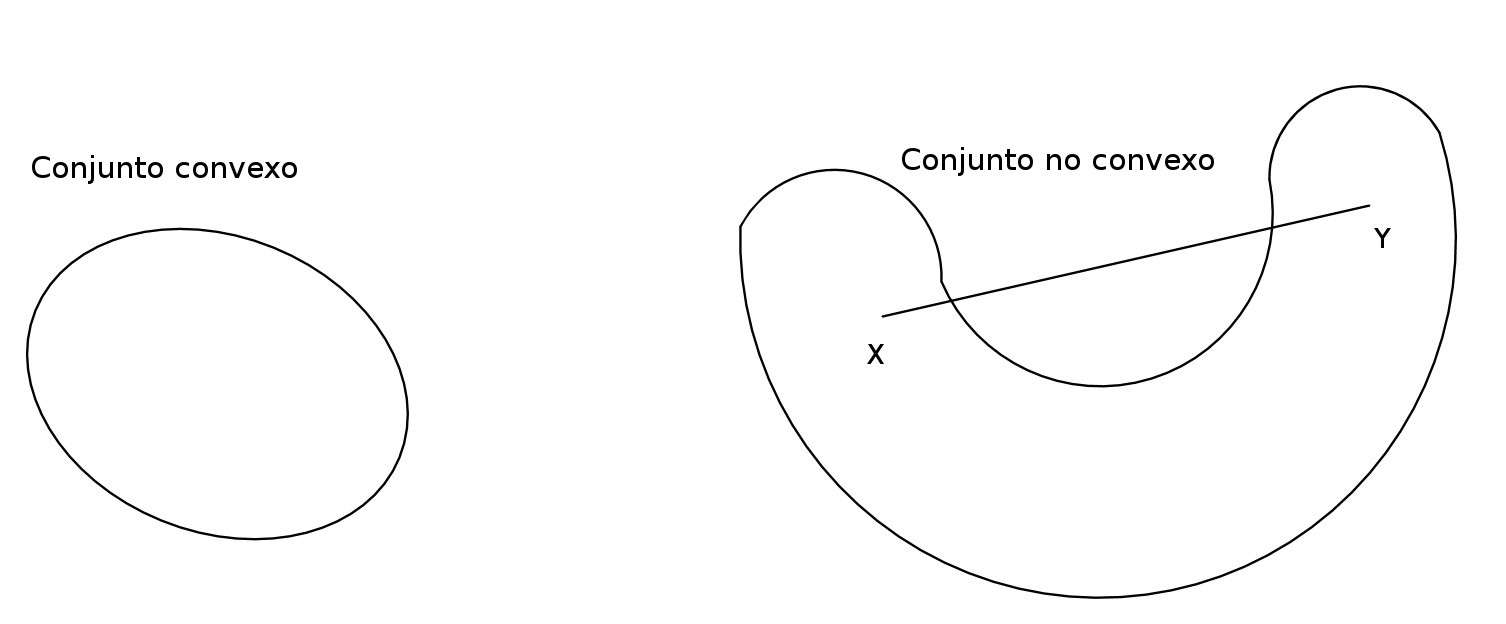
\includegraphics[scale=0.8]{./partes/convexo.jpg}
   \caption{Conjunto convexo y no convexo}
   \label{cyn}
\end{figure}

%--------------------fin de imagen-------------------------------------------------------------

{\definicion: La suma vetorial \cite{no-lineal} 
$$\lambda_1 x_1 + \lambda_2 x_2 + \ldots + \lambda_m x_m$$
es llamada {\bf combinaci\'on convexa} de $x_1, x_2, \ldots , x_m$ si los coeficientes $\lambda_i$
son no negativos y $\displaystyle \sum_{i=1}^{m} \lambda_i = 1$  \label{def2} }\\ \\

% {\corolario: Sea $C \subset X$ un conjunto convexo cerrado no vac\'io del espacio vectorial
% $X$. Entonces, $C$ es la intersecci\'on de todos los semiespacios cerrados que lo contienen, es
% decir:
% \[ C = \bigcap_{C \subset \mathcal{H}_{(z^{*}, \alpha)}}\mathcal{H} _{(z^{*}, \alpha)}\]
% 
% donde $\mathcal{H}_{(z^{*}, \alpha)} := \{x \in X\: \langle x, z^* \rangle \leqslant \alpha \}\, 
% \mbox{para }\, z^* \in Z^* \, \mbox{y} \,\, \alpha \in \mathbb{R}$}
% 
% \medskip \medskip
% 
% {\it{\bf Demostraci\'on.}}\\
% Denotemos por $\mathcal{F}\,$ el conjunto $X^* \times \mathbb{R}$ dado por (notar que es no vac\'io)
% \[\mathcal{F} := \{ (z^*, \, \alpha) \in  X^* \times \mathbb{R} \: C \subset \mathcal{H} 
% _{(z^{*}, \alpha)}\}\]
% 
% Claramente $\displaystyle{ C \subset \bigcap_{\mathcal{F} \subset \mathcal{H}_{(z^{*}, \alpha)}}
% \mathcal{H}_{(z^{*}, \alpha)}}$\\ \\
% 
% Para probar la inclusi\'on inversa tomamos $\displaystyle{ u \in \bigcap_{\mathcal{F} \subset 
% \mathcal{H}_{(z^{*}, \alpha)}} \mathcal{H}_{(z^{*}, \alpha)}}.$\\
% 
% Si $u \notin C $ utilizando el teorema (3) 
% 
% \begin{flushright}
%     $\square$
% \end{flushright}
% 
% \medskip
% 
% {\observacion Los conjuntos cerrados $ \mathcal{H}_{(z^{*}, \alpha)}$ de la proposición anterior también
% resultan ser cerrados para la topolog\'ia d\'ebil y por lo tanto el conjunto convexo cerrado $C$ es 
% cerrado para la topolog\'ia d\'ebil (intersecci\'on de cerrados d\'ebiles). Ası\'i, una conclusi\'on
% importante, y que ser\'a utilizada m\'as adelante, del Corolario (\ref{cor1}), es que todo conjunto convexo cerrado
% es tambi\'en cerrado para la topologı\'ia d\'ebil.}\\
% \medskip

%agregar corolarios que borraste

{\definicion Dado un conjunto $S \subset X$ no vac\'io, diremos que la c\'apsula convexa de $S$ la cual
denotaremos por $Co(S)$, es la intersecci\'on de todos los conjuntos convexos que contienen a $S,$ es decir:
\[Co(S) = \bigcap_{_{S \subset T,\,\, T\, \mbox{\scriptsize convexo}}} T\] \label{cap-convx} }
\medskip

La c\'apsula convexa de un conjunto $S$, $Co(S),$ es convexa. M\'as a\'un, la c\'apsula convexa de un conjunto $S$ es el menor conjunto
convexo que contiene a $S$.\\
\medskip

%------------ imagenes geometricas de cápsula convexa---------------------------------------------------
\begin{figure}[h]
	\centering
	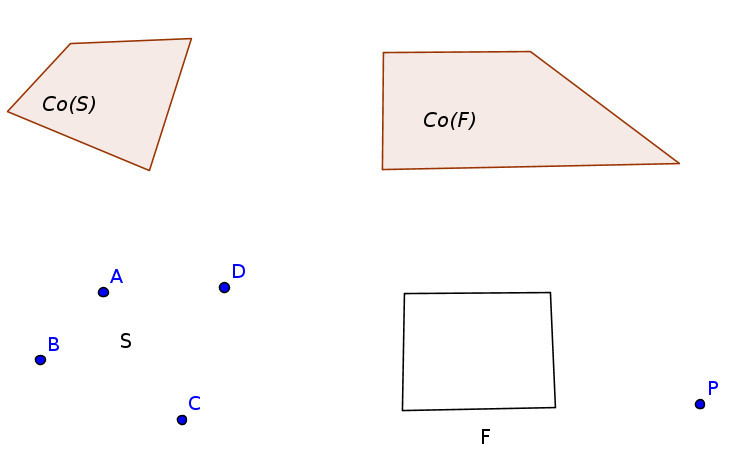
\includegraphics[scale= 1.5]{./partes/capsula_conv.jpg}	
	\caption{C\'apsula convexa}\label{capsula}
\end{figure}\label{capsula}
%---------------------fin de imagenes-------------------------------------------------------------------

{\proposicion La c\'apsula convexa de un conjunto $C \subset X$, no vac\'io, es el conjunto de todas las
combinaciones convexas de elementos de $C$. \label{prop1}}\\ \\

% \textbf{\itshape Demostraci\'on}\\
% Sea $D$ el conjunto de todas las combinaciones convexas de $C$, entonces $C \subset D$ por Corolario(1) $D$ 
% es convexo, por lo tanto $C \subset Co(C) \subset D$.\\
% Rec\'iprocamente, sea $y \in D$, esto implica que $y$ es una combinaci\'on de elementos de $C \subset Co(C)$,
% as\'i $y$ tambi\'en es una combinaci\'on convexa de elementos de $Co(C)$, del Corolario (\ref{cor1}) se
% tiene que $y \in Co(C)$\\ \\
\

Tambi\'en podemos definir la {\it c\'apsula af\'in} de $C$ como la colecci\'on de todas las combinaciones afines
de puntos en $C.$ Esta es la dimensi\'on af\'in m\'as pequeña de un subespacio que contiene a $C$. Por ejemplo: 
la c\'apsula convexa de dos puntos distintos es una recta unidimensional conteniendo estos dos puntos. Similarmente,
la {\it c\'apsula lineal} de $C$ es la colecci\'on de todas las combinaciones lineales de puntos en $C$ \cite{no-lineal}

%------------------------------imagenes de cobertura convexa--------------------------------------------------
% \begin{figure}[h]
% 	\centering
% 	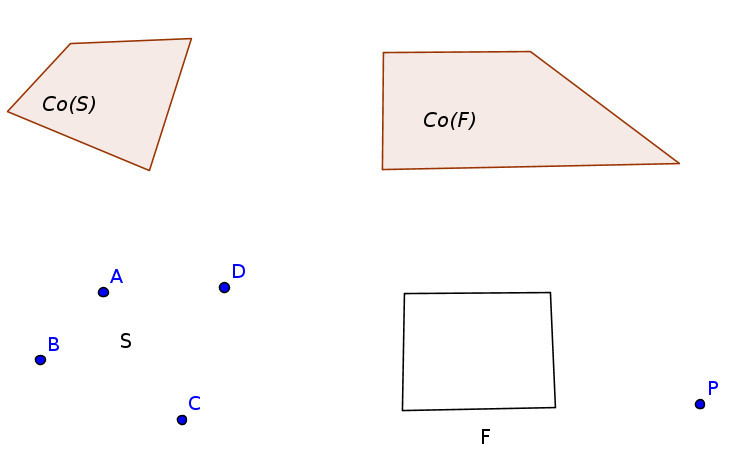
\includegraphics[scale= 1.5]{./partes/capsula_conv.jpg}	
% 	\caption{C\'apsula convexa}\label{capsula}
% \end{figure}\label{capsula}
%-------------------------------------------------------------------------------------------------------------

{\definicion:
\begin{itemize}
   \item La c\'apsula convexa de un n\'umero finito de puntos $x_1, x_2, \ldots ,x_{k+1} \in K$ es llamada politopo.
   \item Si $x_1, x_2, \ldots ,x_{k}\,\,\mbox{y}\,\, x_{k+1} $ son {\itshape independiente afines}, es decir
         que $x_2-x_1,\,x_3-x_1, \ldots , \, x_{k+1}-x_1$ son linealmente independientes, entonces la 
         $Co(x_1, x_2, \ldots ,x_{k+1})$ es llamada un {\itshape simplex} con v\'ertives $x_1, x_2, 
         \ldots ,x_{k+1}$
\end{itemize}
\label{def-poli-simplex}
}

La figura \ref{im2} nos muestra un ejemplo de un politopo y un simplex en $\mathbb{R}^n$. Note que el n\'umero
m\'aximo de vectores linealmente independientes en $\mathbb{R}^n \,\, \mbox{es}\,\, n$ y por lo tanto no
podr\'ia haber ning\'un simplex en $\mathbb{R}^n$ teniendo m\'as de $n+1$ v\'ertices.

%------------------------------------figura de definicion anterior--------------------------------------------

\begin{figure}
   \centering
   \begin{center}

\definecolor{zzttqq}{rgb}{0.6,0.2,0}
\definecolor{qqqqff}{rgb}{0,0,1}
\begin{tikzpicture}[line cap=round,line join=round,>=triangle 45,x=1.0cm,y=1.0cm]
\clip(0.3,2.48) rectangle (11.74,8.56);
\fill[color=zzttqq,fill=zzttqq,fill opacity=0.1] (1.3,7.1) -- (0.44,5.4) -- (2.62,4.06) -- (4.78,5.16) -- (4.84,7.42) -- cycle;
\fill[color=zzttqq,fill=zzttqq,fill opacity=0.1] (7.82,7.2) -- (7.12,4.74) -- (11.16,5.28) -- cycle;
\draw [color=zzttqq] (1.3,7.1)-- (0.44,5.4);
\draw [color=zzttqq] (0.44,5.4)-- (2.62,4.06);
\draw [color=zzttqq] (2.62,4.06)-- (4.78,5.16);
\draw [color=zzttqq] (4.78,5.16)-- (4.84,7.42);
\draw [color=zzttqq] (4.84,7.42)-- (1.3,7.1);
\draw [color=zzttqq] (7.82,7.2)-- (7.12,4.74);
\draw [color=zzttqq] (7.12,4.74)-- (11.16,5.28);
\draw [color=zzttqq] (11.16,5.28)-- (7.82,7.2);
\draw (2,6.24) node[anchor=north west] {Politopo};
\draw (8,6.24) node[anchor=north west] {Simplex};
\begin{scriptsize}
\fill [color=qqqqff] (1.3,7.1) circle (1.5pt);
\draw[color=qqqqff] (1.46,7.36) node {$A$};
\fill [color=qqqqff] (0.44,5.4) circle (1.5pt);
\draw[color=qqqqff] (0.6,5.66) node {$B$};
\fill [color=qqqqff] (2.62,4.06) circle (1.5pt);
\draw[color=qqqqff] (2.78,4.32) node {$C$};
\fill [color=qqqqff] (4.78,5.16) circle (1.5pt);
\draw[color=qqqqff] (4.94,5.42) node {$D$};
\fill [color=qqqqff] (4.84,7.42) circle (1.5pt);
\draw[color=qqqqff] (5,7.68) node {$E$};
\fill [color=qqqqff] (7.82,7.2) circle (1.5pt);
\draw[color=qqqqff] (7.96,7.46) node {$F$};
\fill [color=qqqqff] (7.12,4.74) circle (1.5pt);
\draw[color=qqqqff] (7.28,5) node {$G$};
\fill [color=qqqqff] (11.16,5.28) circle (1.5pt);
\draw[color=qqqqff] (11.32,5.54) node {$H$};
\end{scriptsize}
\end{tikzpicture}\end{center}
   \caption{Politopo y simplex}\label{figure: Politopo y Simplex}
   \label{im2}
\end{figure} 

%-------------------------------------------------------------------------------------------------------------
%agrega teorema que borraste
{\corolario $C_1 \subset C_2 \Longrightarrow co(C_1) \subset co(C_2)$}\label{cor2}\\ \\
\

\textbf{Teorema de Caratheodory \cite{no-lineal}} 

Por definici\'on, un punto en el conjunto de una c\'apsula convexa puede ser representado coomo una
combinaci\'on convexa de un n\'umero finito de puntos en el conjunto. El siguiente teorema muestra 
que cualquier punto $x$ en la c\'apsula convexa de un conjunto $C$ puede ser representado como una 
combinaci\'on de a lo sumo $n+1$ puntos en $C$. El teorema es trivialmente cierto para $x\in C$.

{\teorema: Sea $C$ un conjunto arbitrario en $\mathbb{R}^n$. Si $x \in Co(C),\,\, x \in Co(x_1, \ldots , x_{n+1})$ donde
$x_j \in C,\,\mbox{para}\,\, j=1, \ldots , n+1.$ En otras palabras $x$ se puede representar como:

\begin{eqnarray*}
   x = \sum_{j=1}^{n+1} \lambda_j x_j\mbox{;} & x_j \in C\,\, \mbox{para}\,\, j=1, \ldots, n+1 \\  
   \sum_{j=1}^{n+1} \lambda_j = 1\mbox{;} & \lambda_j \geqslant 0 \,\,\mbox{para}\,\, j=1, \ldots, n+1
\end{eqnarray*}
\label{teo-carateodory} }

%\newpage
\subsection{Propiedades topol\'ogicas de los conjuntos convexos}

A continuaci\'on desarrollaremos algunas propiedades topol\'ogicas para conjuntos convexos \cite{no-lineal}. Como 
un preliminar a esta parte tendremos que dado un punto $x \in \mathbb{R}^n$ un 
$\varepsilon$-vecindario alrededor del conjunto es $N_{\varepsilon}(x)= \{y: \parallel y - x \parallel < \varepsilon\}$.
Primero revisaremps las definiciones de: clausura, interior y frontera de un conjunto arbitrario en $\mathbb{R}^n$,
usando el concepto de $\varepsilon-$vecindario.\\

{\definicion: Sea $S$ un conjunto arbitrario en $\mathbb{R}^n$. 
\begin{itemize}
   \item {\bf Clausura}: Se dice que un punto $x \in \mathbb{R}^n$ est\'a en la clausura de $S$ si \linebreak
	 $\forall \, \varepsilon > 0, \,\,\,\,S\cap N_{\varepsilon}(x) \neq \emptyset $
   \item {\bf Interior}:Un punto $x$ se dice que est\'a en el interior de $S$ si \linebreak
	 $\exists \varepsilon > 0$\, tal que $N_{\varepsilon}(x) \subset S$.
   \item {\bf Frontera}: Un punto $x$ se dice que est\'a en la frontera si $\forall \, \varepsilon > 0$ se tienen que \linebreak
	 $N_{\varepsilon}(x) \cap S \neq \emptyset\,$ y $\,N_{\varepsilon}(x) \cap S^{c} \neq \emptyset$
   \item {\bf Acumulaci\'on}: Un punto $x$ es de acumulaci\'on de $S$ si \linebreak
	 $\forall \,\, \varepsilon > 0$ se tiene que $(N_{\varepsilon}(x)-\{x\}) \cap S \neq \emptyset$
\end{itemize}
\label{top-notable}}

\medskip

\textbf{Notaci\'on:}
\begin{itemize}
   \item Denotaremos por $\, \overline{S}$ a la clausura del conjunto $S$. Adem\'as se tiene que $S$ es cerrado si $\overline{S} = S$.
   \item Denotaremos por $\, \mathring{S}$ al interior del conjunto $S$ y \'este es abierto cuando $\mathring{S}=S$
   \item Denotaremos por $\,fr(S)$ a la frontera del conjunto $S$.
   \item Denotaremos por $\, S'$ al conjunto de puntos de acumulaci\'on de $S$
\end{itemize}

\medskip

Finalmente, un conjunto es acotado si puede ser contenido en una bola bola de radio suficientemente grande. Un conjunto es 
{\itshape compacto} si es cerrado y acotado. Note que el complememeto de un conjunto abierto en un conjunto cerrado (viceversa)
y que los puntos de acumulaci\'on de cualquier conjunto y su complemento son el mismo.\\

\medskip

una manera un poco m\'as f\'acil de asimilar \'estas definiciones es de forma gr\'afica considerando
$S = \{(x, y): x^2 + y^2 \leqslant 1\}$, este conjunto representa todos los puntos dentro del circulo con centro $C(0, 0)$ y 
radio $r=1$. (V\'ease \ref{top})\\

F\'acilmente se puede verificar que $S$ es cerrado, es decir, $\overline{S} = S$.\\
Adem\'as $\mathring{S}$ consiste en todos los puntos que est\'an estrictamente dentro del circulo, esto es,
$\mathring{S} = \{(x, y): x^2 + y^2 < 1 \}$.\\
Finalmente, $S'$ consiste de los puntos en el circulo, esto es, $S' = \{(x, y): x^2 + y^2 = 1\}$.

%------------------------------------topologia de un conjunto--------------------------------------------------------------------
\begin{figure}[h]
  \centering
  \subfigure[Cerradura $\overline{S}$]{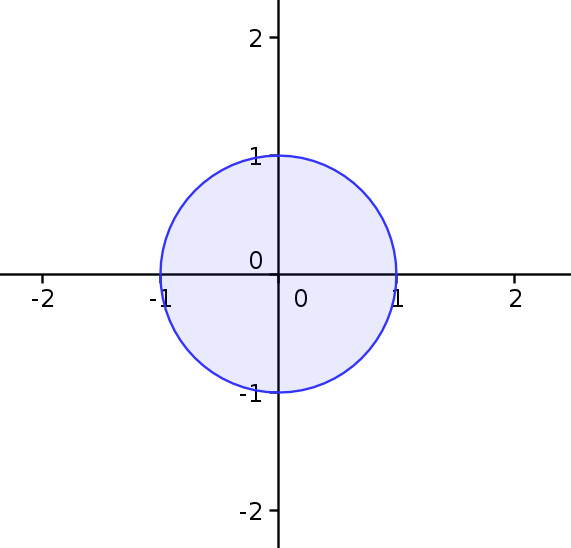
\includegraphics[scale = 1]{./partes/sub_sec/topo.jpg}}
  \subfigure[Interior $\mathring{S}$]{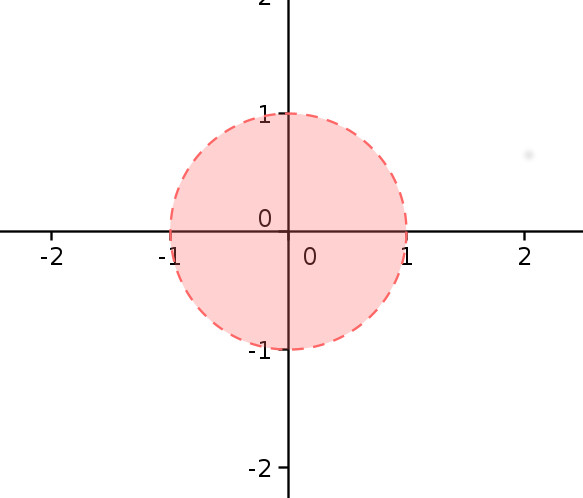
\includegraphics[scale = 1]{./partes/sub_sec/topo_cl.jpg}}
  \subfigure[Acumulaci\'on $S'$]{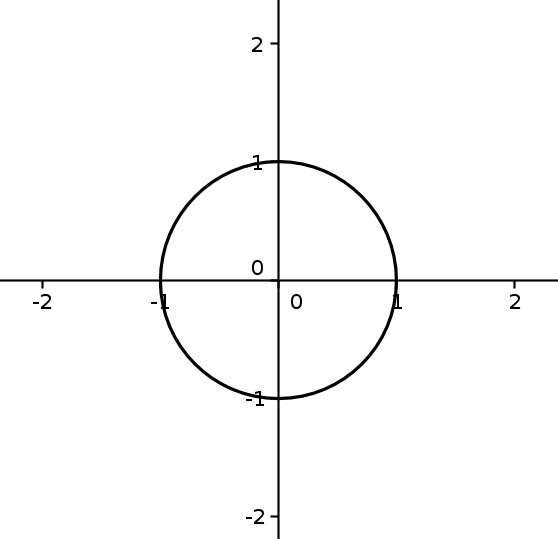
\includegraphics[scale = 1]{./partes/sub_sec/topo_ac.jpg}}
  \caption{Topolog\'ia del conjunto $S = \{(x, y): x^2 + y^2 \leqslant 1\}$}
\end{figure}\label{top}

%---------------------------------------------------------------------------------------------------------------------------------

~\\ \\

\textbf{Caracterizaciones de conjuntos}\\

\begin{itemize}%verificar que item 3 sea abierto
   \item Un conjunto $S$ es cerrado si y solo si contiene todos sus puntos de acumualci\'on, es decir $S' \subset S$.
   \item $\overline{S} = S \cup S'$ es el cerrado m\'as peque\~no que contiene al conjunto $S$.
   \item Un conjunto $S$ es abierto si y solo si \'este no contiene ninguno de sus puntos frontera, mas precisamente $S' \cap S = \emptyset$.
   \item $\mathring{S} \subseteq S$, por la tanto, tenemos que $\mathring{S} = S - S'$ mientras que necesariamente
	$S' \neq S - \mathring{S}$.
\end{itemize}

Un conjunto puede ser ni abierto ni cerrado, los \'unicos conjuntos que son abiertos y cerrados a la vez son el conjunto vac\'io
($\emptyset$) y el mismo $\mathbb{R}^n$. Tambi\'en consideremos que ning\'un punto $\overline{x} \in S$ puede ser un punto interior o de 
acumulaci\'on de $S$. Sin embargo $S \neq \mathring{S} \cup S'$, es decir que $S$ no necesita contener sus puntos de acumulaci\'on.\\ 

Existe otra definici\'on equivalente de conjunto cerrado, el cual es muy importante demostrando desde el punto de vista que es un
conjunto cerrado.\\Esta definici\'on est\'a basada en las sucesiones de puntos contenidos en $S$. \\
Un conjunto es cerrado si y solo si para cualquier sucesi\'on convergente de puntos $\{ x_k \} _{k \in \mathbb{N}} \in S$ con punto
l\'imite $\overline{x}$, as\'i mismo tenemos que $\overline{x} \in S$.\\
La equivalencia de \'esta y la definici\'on previa de cerradura es f\'acilmente de ver ya que el punto l\'imite $\overline{x}$ de 
cualquier sucesi\'on convergente de puntos en $S$ debe encontrarse en el interior o de acumulaci\'on de $S$, en otras palabras
deber\'ia existir un $\varepsilon > 0$ tal que $\{x: \parallel x - \overline{x} \parallel < 0 \} \cap S = \emptyset$ contradiciendo
que $\overline{x}$ es el punto l\'imite de una sucesi\'on contenida en $S$.\\

%llevar un mejor orden en la parte topolog\'ia y ya aplicado a conjuntos convexos y esta otra

\textbf{Segmento de linea entre puntos del interior y cerradura de un conjunto \cite{no-lineal}}\\

Dado un conjunto convexo con interior no vac\'io, el segmento de linea (excluyendo los puntos finales) que une un punto del interior
del conjunto con un punto de la clausura de este pertenece al interior del conjunto. Este resultado se muestra acontinuaci\'on.\\


{\teorema Sea $S$ un conjunto convexo en $\mathbb{R}^n$ con interior no vac\'io. Sea $x_1 \in \overline{S}\,$ y $\, x_2 \mathring{S}$.
Entonces $\lambda x_1 + (1 - \lambda)x_2 \in \mathring{S}~\,\,\, \forall \,\,\,\, \lambda \in (0, 1)$ \label{t_int}}\\

\textbf{\itshape Demostraci\'on: }\\
Como $x_2 \in \mathring{S}\,$ existe un $\varepsilon > 0$ tal que $\{z: \parallel z - x_2 \parallel < \varepsilon\} \in S$. Sea $y$ tal que

\begin{equation}
   y = \lambda x_1 + (1 - \lambda)x_2;~ \lambda \in (0, 1)
   \label{convx}
\end{equation}


Para probar que $y \in \mathring{S}$ es suficiente construir un vecindario sobre $y$ que tambi\'en pertenece a $S$. En particular 
mostraremos que $\{z: \parallel z - y \parallel < (1 - \lambda)\varepsilon\}.$ Sea $z$ tal que 
$\parallel z - y \parallel < (1 - \lambda)\varepsilon$ (v\'ease \ref{convx}), ahora bien, como $x_1 \in \overline{S}$

\[\left \{x: \parallel x - x_1 \parallel < \dfrac{(1 - \lambda)\varepsilon - \parallel z - y \parallel}{\lambda} \right \} \cap S\]

es no vac\'io, en particular, existe $z_1 \in S$ tal que 

\begin{equation}
   \parallel z_1 - x_1 \parallel < \displaystyle{\dfrac{(1 - \lambda)\varepsilon - \parallel z - y \parallel}{\lambda}} 
   \label{casi}
\end{equation}


Ahora, sea $z_2 = \dfrac{z - \lambda z_1}{1 - \lambda}$ de (\ref{convx}), la desigualdad de Schwartz y (\ref{casi}) tenemos: 

\begin{eqnarray*}
   \parallel z_2 - x_2 \parallel = \parallel \dfrac{z - \lambda z_1}{1 - \lambda} - x_2 \parallel &=& \displaystyle{\parallel \dfrac{(z - \lambda z_1) - (y - \lambda x_1)}{1 - \lambda} \parallel} \\  
   &=& \dfrac{1}{1 - \lambda} \displaystyle{ \left\| (z - y) + (x_1 - \lambda x_1) \right\|} \\
  & \leqslant & \dfrac{1}{1 - \lambda} (\parallel z - y \parallel + \lambda \parallel x_1 - z_1 \parallel)\\
  &<& \varepsilon
\end{eqnarray*}

Por lo tanto, $z_2 \in S.$ Dada la definici\'on de $z_2$ notemos que  $z = \lambda z_1 + (1 - \lambda)z_2$, como $z_1\,$ y $\, z_2$
pertenecen a $S$, entonces $z$ tambi\'en pertenece a $S$. Hemos mostrado que para cualquier $z$ con $\parallel z - y \parallel < 
(1 - \lambda)\varepsilon$ pertenece a $S$. Por lo tanto $y \in \mathring{S}. \\$ 
\begin{flushright}
  $\square$ 
\end{flushright}


{\corolario Sea $S$ un cojunto convexo. Entonces $\mathring{S}$ es convexo. \label{int-convx}}

{\corolario Sea $S$ un conjunto convexo con interior no vac\'io. Entonces $\overline{S}$ es convexa. \label{cl-convx}}\\

\textbf{\itshape Demostraci\'on}\\
Asumiendo que $\mathring{S} \neq \emptyset$. Sea $x_1, x_2 \in \overline{S}$, por teorema tenemos que 
$$\lambda x_2 + (1 - \lambda)z \in \mathring{S}\,\,\,\, \forall \,\,\lambda \in (0, 1)$$

Sea $\mu \in (0, 1)\,$ fijo. Por teorema \ref{t_int}:
$$\mu x_1 + (1 - \mu)[\lambda x_2 + (1 - \lambda)z] \in \mathring{S} \subset S \,\,\,\, \forall \, \lambda \in (0, 1)$$

Si tomamos el l\'imite cuando $\lambda $ se apr\'oxima $1$ se tiene que: $\mu x_1 + (1 - \mu)x_2 \in \overline{S}.$
\begin{flushright}
   $\square$
\end{flushright}

{\corolario Sea $S$ un conjunto convexo con interior no vac\'io. Entonces $\overline{(\mathring{S})} = \overline{S}$. \label{cl}}\\

\textbf{\itshape Demostraci\'on}\\
Claramente $\overline{(\mathring{S})} \subseteq \overline{S}.$ Sea $x \in \overline{S}\,$ escogemos $y \in \mathring{S}$ (asumieno que
$\mathring{S} \neq \emptyset\, $). Entonces:

$$\lambda x + (1 - \lambda)y \in \mathring{S}\,\,\,\, \forall \, \lambda \in (0, 1)$$

Haciendo $\lambda \rightarrow 1^{-} $ se sigue que $x \in \overline{(\mathring{S})}.$
\begin{flushright}
   $\square$
\end{flushright}

{\corolario Sea $S$ un conjunto convexo con interior no vac\'io. Entonces $\mathring{(\overline{S})} = \mathring{S}$ \label{int} }\\

\textbf{\itshape Demostraci\'on:}\\
Note que $\mathring{S} \subseteq \mathring{(\overline{S})}. $ Sea $x_1 \in \mathring{(\overline{S})}$, necesitamos mostrar que 
$x \in \mathring{S}$. Existe un $\varepsilon > 0 $ tal que $\parallel y - x_1 \parallel < \varepsilon$ implica que $y \in \overline{S}$.
Ahora, sea $x_2 \neq x_2 \in \mathring{S}$ y sea $y = (1 + \delta)x_1 - \delta x_2$, donde $\delta = 
\dfrac{\varepsilon}{2\parallel \parallel}$. Como $\parallel \parallel = \dfrac{\varepsilon}{2}, \,\, y \in \overline{S}$. Pero

$$\lambda = \dfrac{1}{1 + \delta} \in (0, 1)$$

Como $y \in \overline{S} $ y $x_2 \in \mathring{S} $ entonces por teorema \ref{t_int}, $x_1 \in \mathring{S}$
\begin{flushright}
   $\square$
\end{flushright}









 %						topologia de conjuntos convexos%
% \newpage
\subsection{Teorema de Weierstrass}

Un resultado muy importante y ampliamente utilizado se basa en los conceptos anteriores. Este resultado relaciona la existencia de una 
soluci\'on de minimizaci\'on para un problema de optimizaci\'on \cite{no-lineal}. 

\begin{itemize}
   \item Podemos decir que $\overline{x}$ es una soluci\'on de minimizaci\'on al problema $\min \{f(x); x \in S \}$, siempre que 
	 $\overline{x} \in S $ y $ f(\overline{x}) \leqslant f(x)\,\,\,\, \forall \, x \in S$. En tal caso, decimos que existe un m\'inimo.
   \item Por otra parte, decimos que $ \alpha = \inf \{ f(x)| x \in S \} $ si $\alpha $ es la mayor de las cotas inferiores de $ f $ en 
	 $ S; $ estos es: $ \alpha \leqslant f(x) \,\,\, \forall \,\, x\in S $ es decir que no hay $\overline{\alpha} > \alpha$ 
	 tal que $ \overline{\alpha} \leqslant f(x) \,\,\, \forall \, x \in S. $
   \item Similarmente, $\alpha = \max \{ f(x)| x \in S \} $ si existe una soluci\'on $ \overline{x} \in S $ tal que 
	 $\alpha = f(\overline{x}) \geqslant f(x) \,\,\, \forall \, x \in S.$
   \item Por otro lado, $\alpha = \sup \{ f(x)| x \in S \} $ si $ \alpha $ es la menor de las cotas superiores de $ f $ en $ S; $ esto es 
	 $ \alpha \geqslant f(x) \,\,\, \forall \, x \in S, $ y no hay otro $\overline{\alpha} < \alpha $ tal que
	 $ \overline{\alpha} \geqslant f(x) \,\,\, \forall \, x \in S$
\end{itemize}


En la Figura (\ref{no_sol}) se ilustran tres momentos en los que el m\'inimo no existe. \\
En la Figura (\ref{no_sol}a) el \'infimo de de $ f $ sobre $(a, b) $ est\'a dado por $f(b)$ pero como $S$ no es cerrado y en particular
$b \notin S$ el \'inimo no existe.\\
En la Figura (\ref{no_sol}b) tenemos que $\inf \{ f(x);\, x \in [a, b]\} $ es\'a dado por el l\'imite de $f(x)$ cuando x tiende a $b$ por
la izquierda. ($\displaystyle{\lim_{x \rightarrow b^{-}} f(x)}$). Como $f$ es discontinua en $b$ no existe una soluci\'on de minimizaci\'on.\\
La figura (\ref{no_sol}c) ilustra cuando $f $ no es acotada sobre un conjunto $S = \{x: \ x \geqslant a \}$

%------------------------------figura de maximo y minimo-------------------------------

\begin{figure}
   \centering
   \subfigure[$S$ es no cerrado]{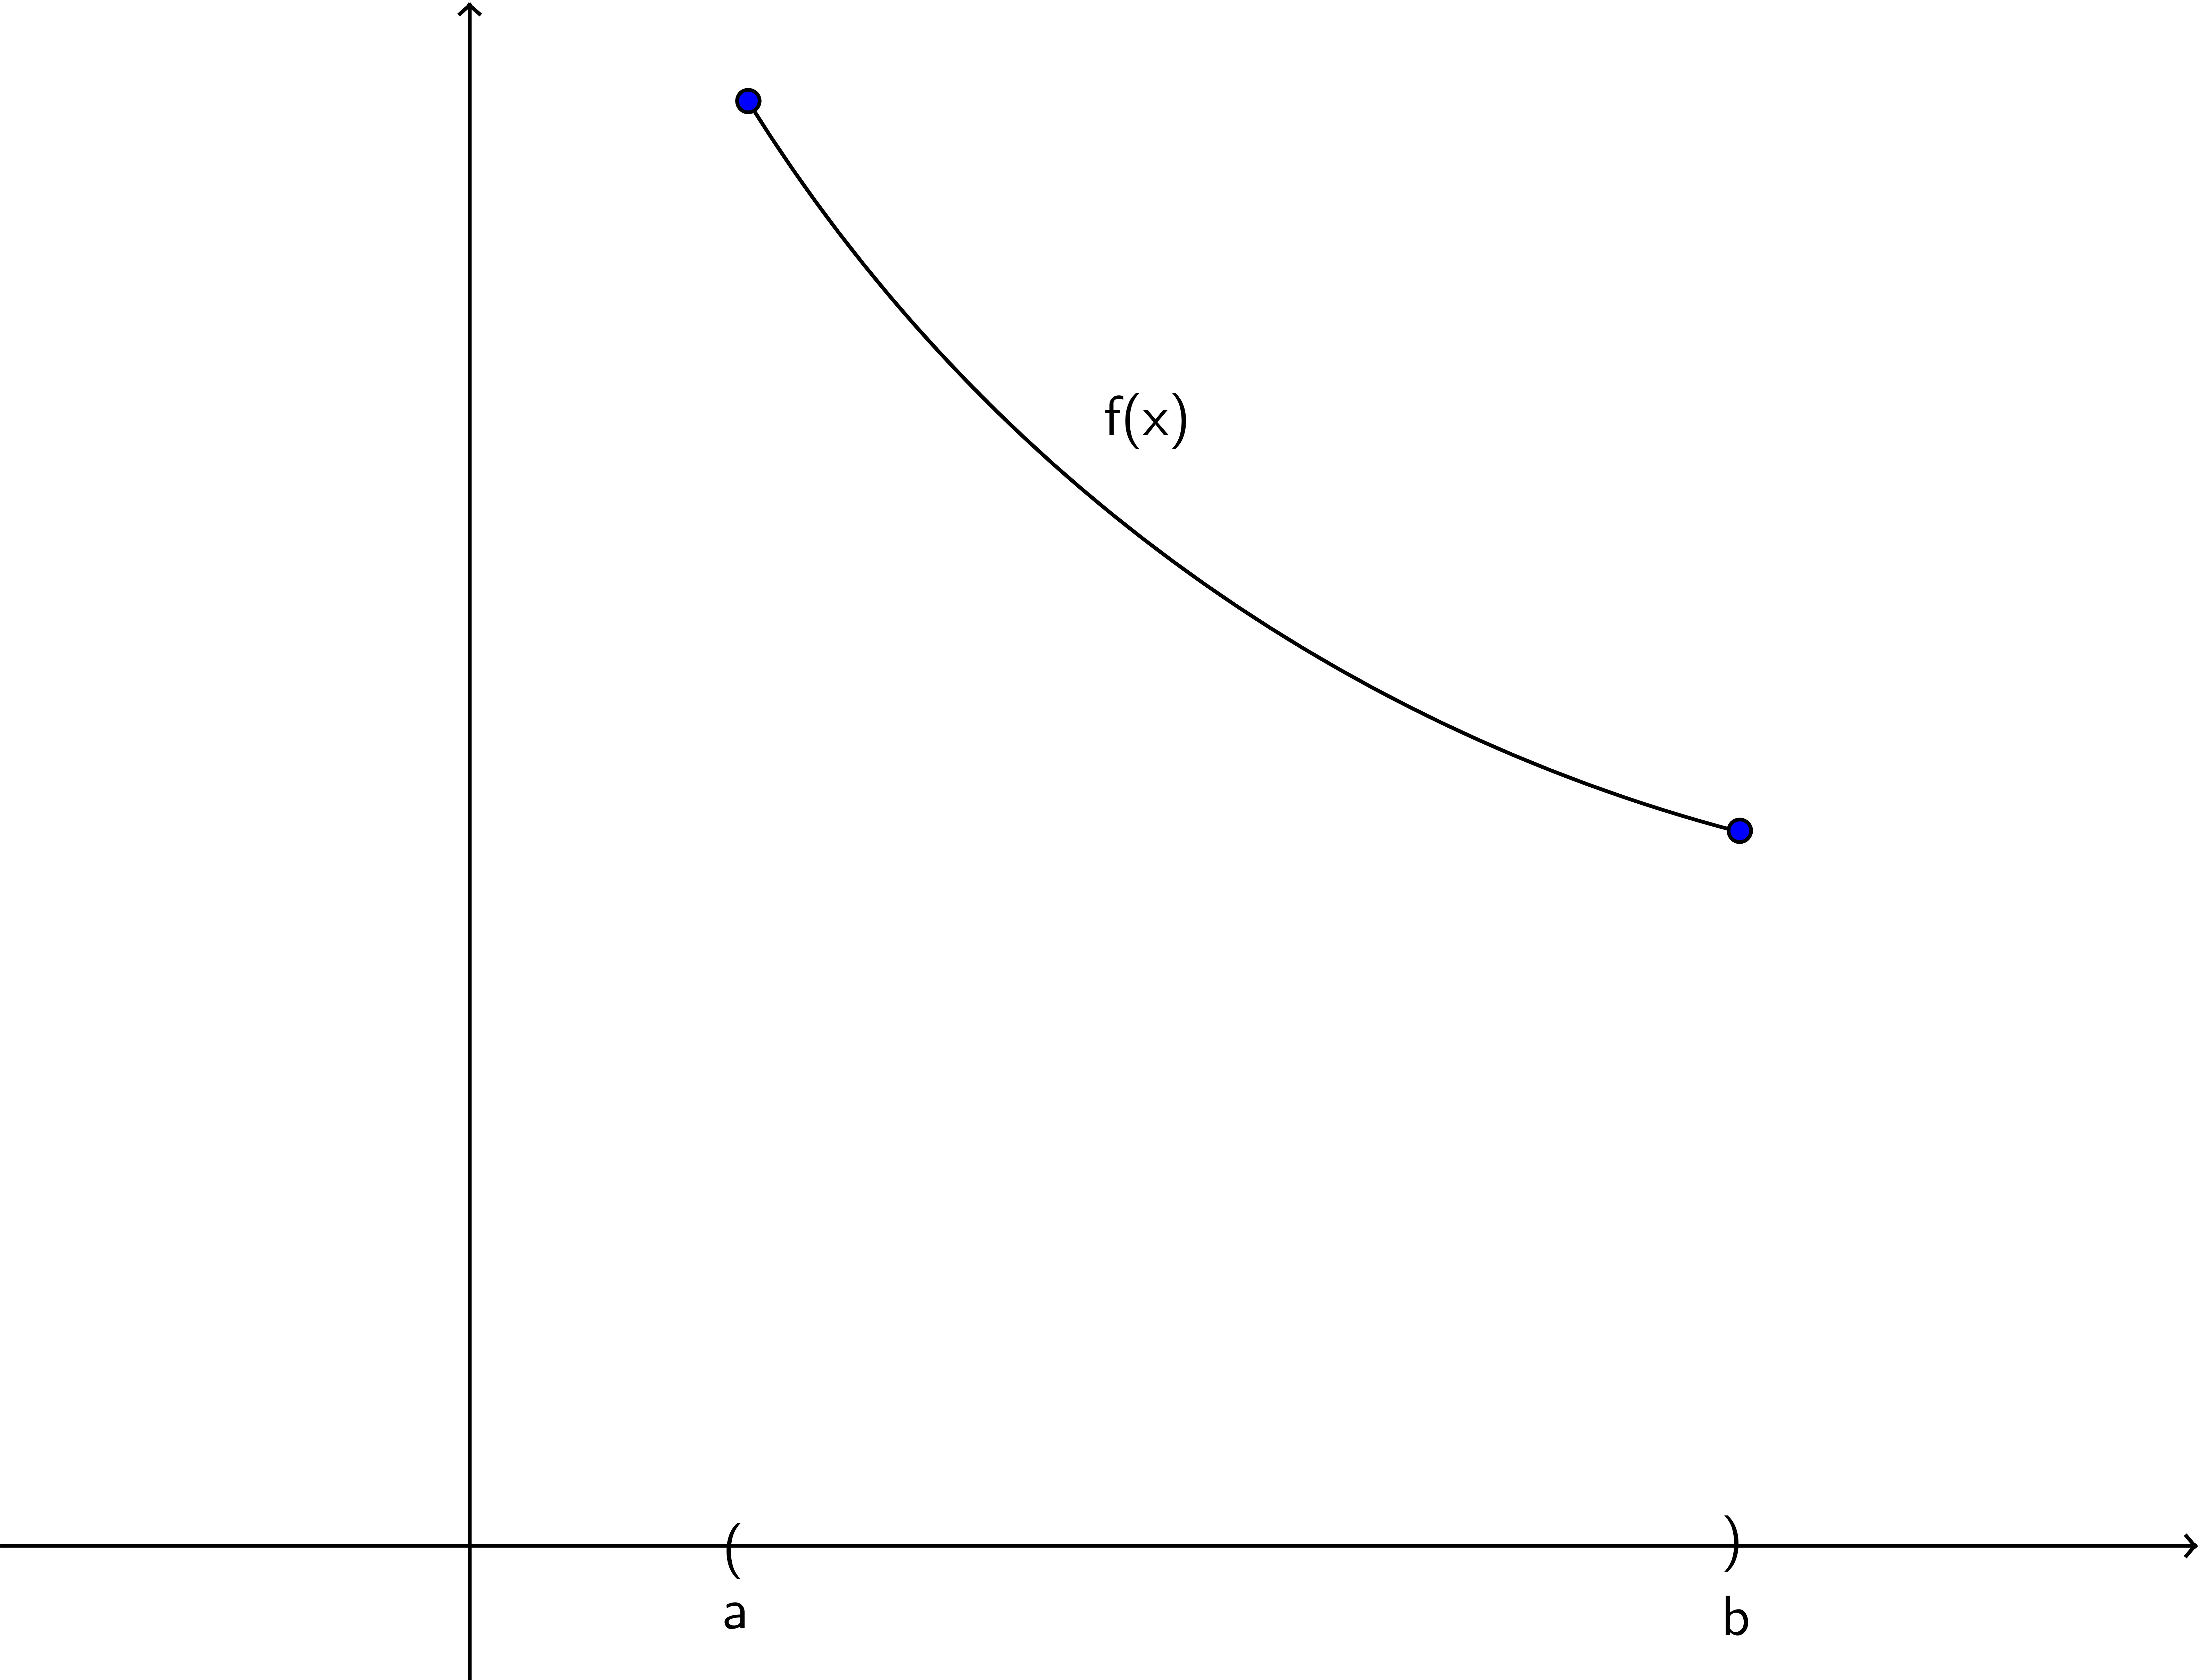
\includegraphics[scale = 0.1]{./partes/sub_sec/2_5a.jpg}}
   \subfigure[$f$ discontinua]{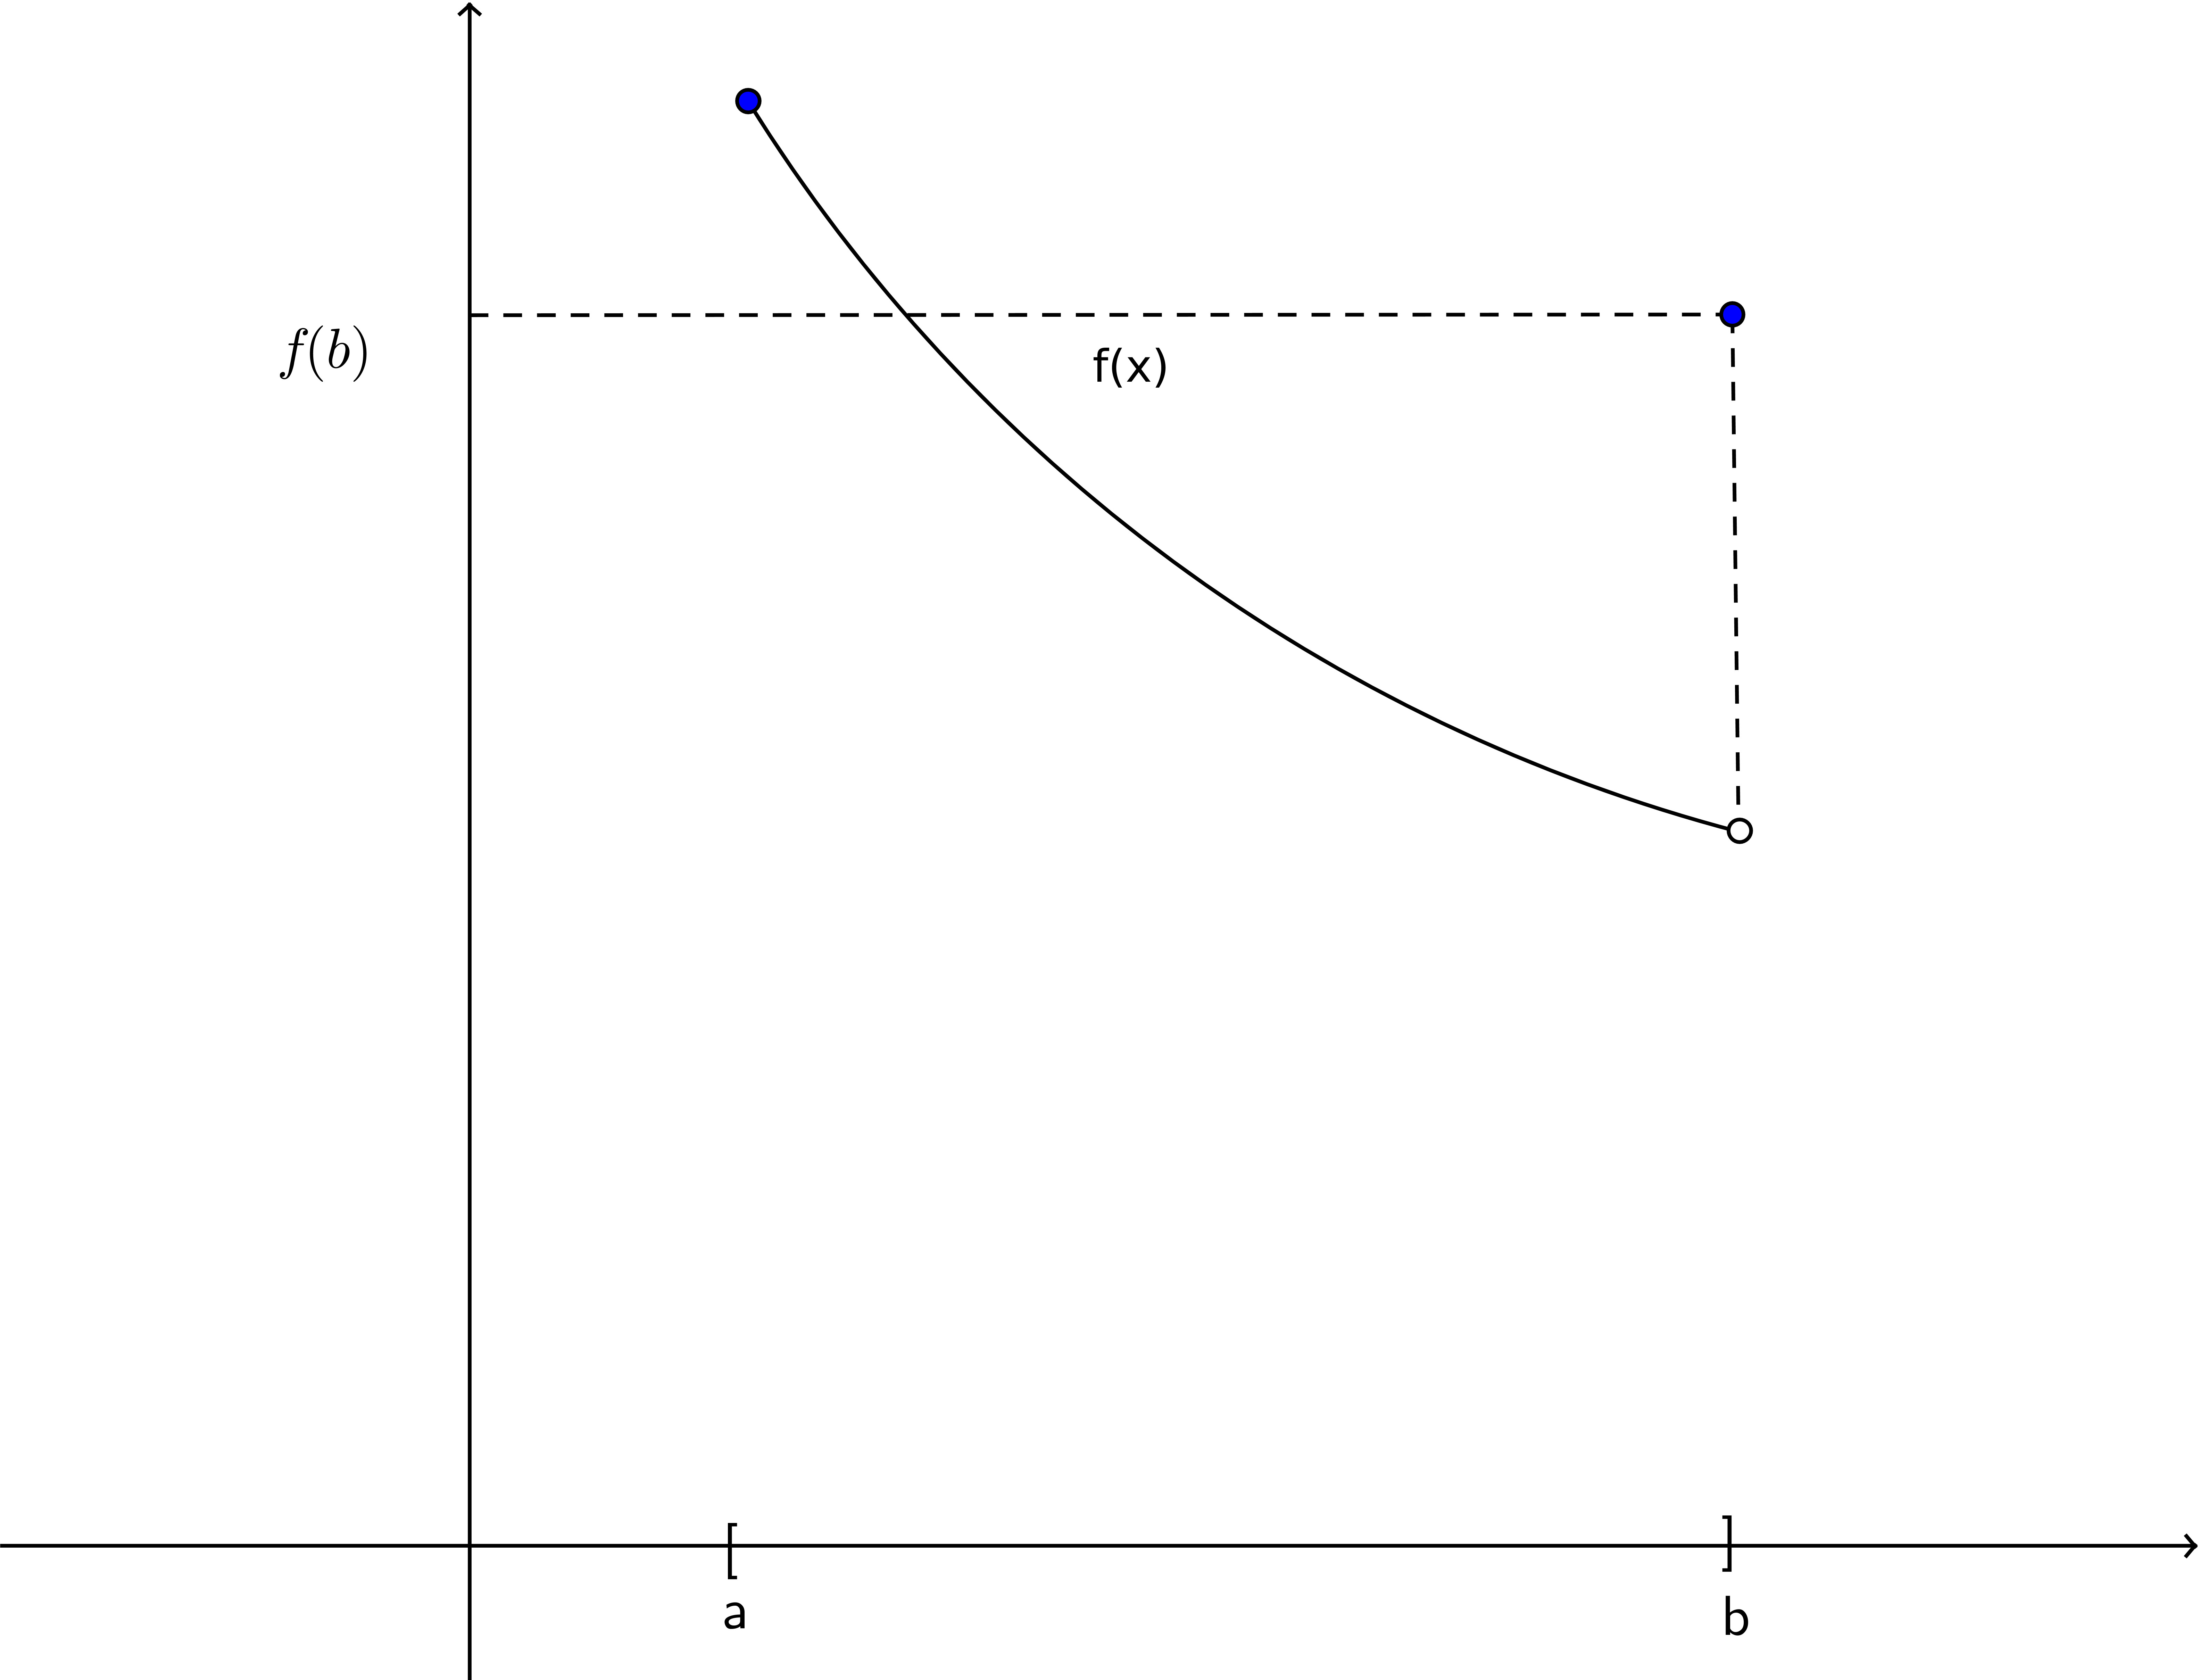
\includegraphics[scale = 0.1]{./partes/sub_sec/2_5b.jpg}}
   \subfigure[$f$ no acotada]{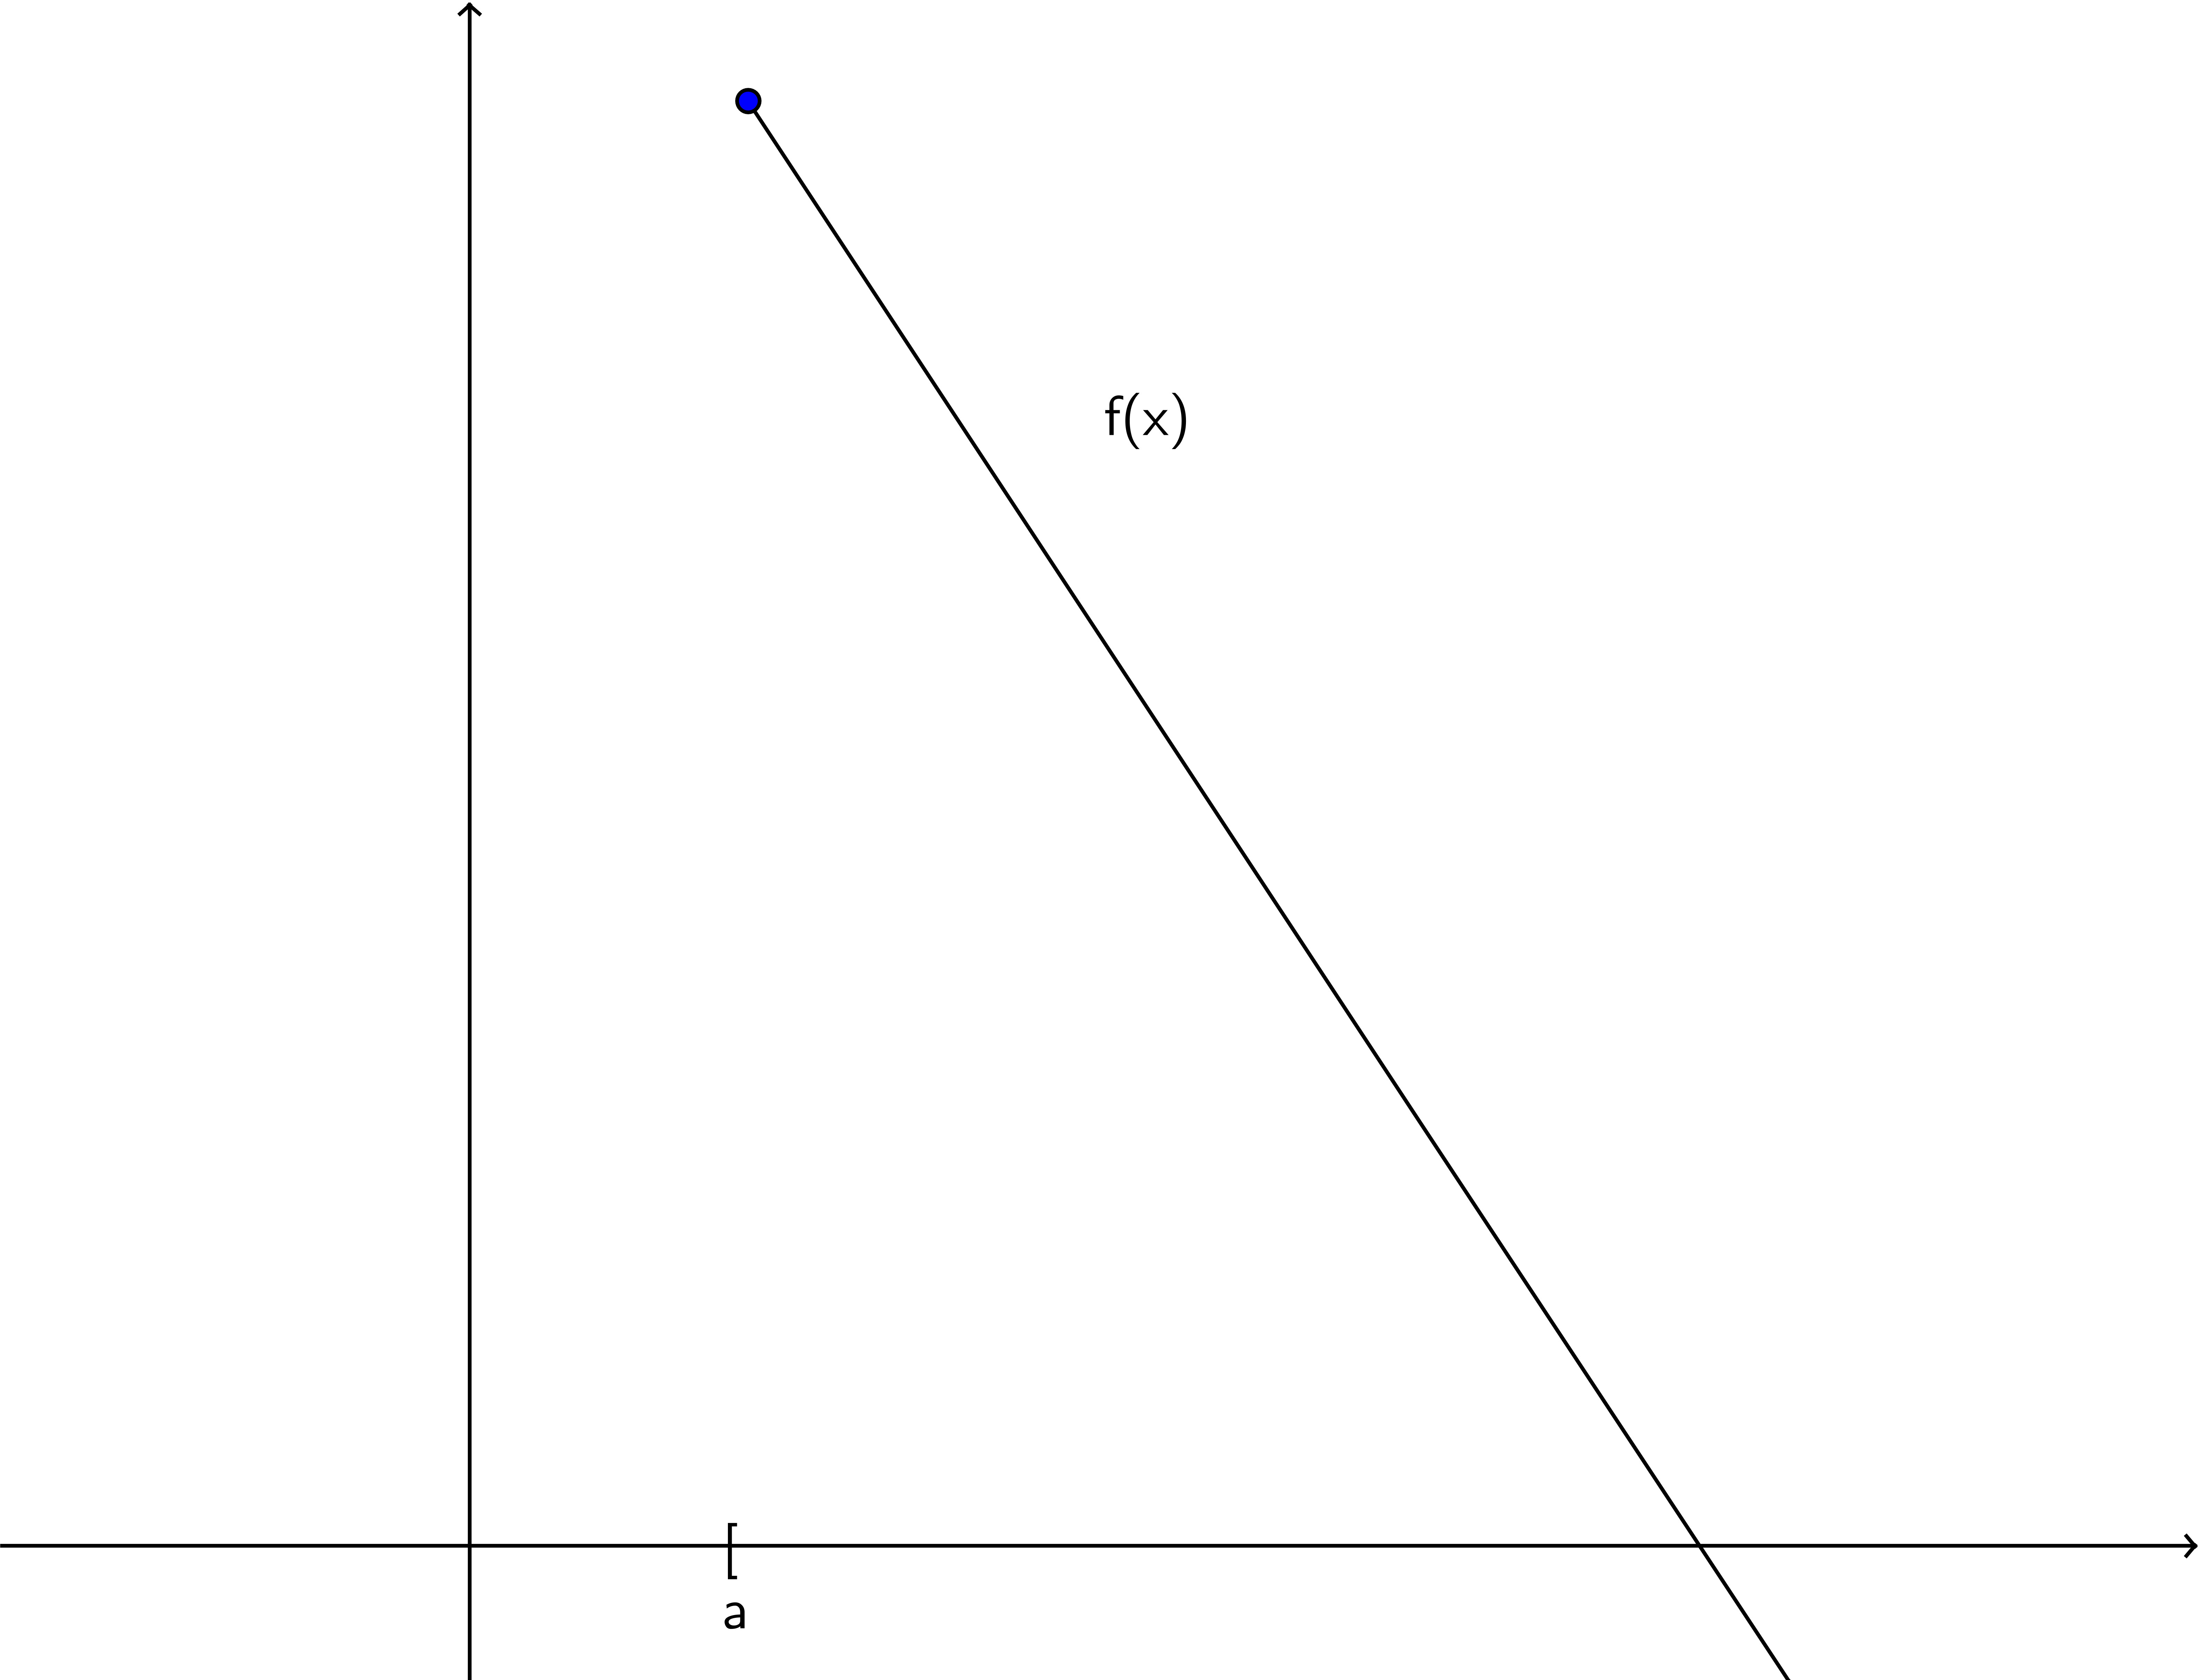
\includegraphics[scale = 0.1]{./partes/sub_sec/2_5c.jpg}}
   \caption{Inexistencia de soluci\'on de minimizaci\'on \cite{no-lineal}}
   \label{no_sol}
\end{figure}

%---------------------------------------------------------------------------------------

Ahora probaremos formalmente este resultado cuando $S$ es no vaci\'o, cerrado y acotado, $f$ continua en $S$, con \'estas condiciones
el m\'inimo en la Figura \ref{no_sol} si existe.\\

{\teorema Sea $S$ un conjunto no vac\'io, compacto y sea $f \longmapsto \mathbb{R}$ continua en $S$ entonces el problema
$\min \{f(x): x \in S\}$ alcanza su m\'inimo; esto es, existe una solucion de minimizaci\'on para este problema. \label{sol-min}}\\

\textbf{\itshape Demostraci\'on:}\\

Como $f$ es continua en $S$ y $S$ es cerrado y acotado, $f$ tambi\'en est\'a acotada (recordar que $f$ es continua), como $S \neq \emptyset$,
existe una cota inferior (la m\'as grande) $\alpha \equiv \min \{f(x):\, x \in S\}$. Ahora, sea $0 < \varepsilon < 1$ y consideremos el
conjunto $S_{k} = \{x \in S:\, \alpha \leqslant f(x) \leqslant \alpha + \varepsilon^{k}\}\,\, \forall\, k=1,\, 2, \ldots .$ Por la 
definici\'on de m\'inimo se tiene que $S_{k} \neq \emptyset \,\,\, \forall \, k$, entonces, tambi\'en podemos construir una sucesi\'on de puntos
$\{x_k\} \subseteq S$ seleccionando un punto $x_k \in S_k\,\, \forall \, k =1,\,2, \ldots $ Como $S$ es acotado, existe existe una
subseci\'on convergente $\{x_k \}_{K}\rightarrow \overline{x}$ indexada por el conjunto $K$. Por la cerradura de $S$ tenemos
$\overline{x} \in S$; y por la continuidad $f$ se tiene que como  $\alpha \leqslant f(x) \leqslant \alpha + \varepsilon^{k} \,\, \forall\, k$
tenemos que:

$$\alpha = \displaystyle{\lim_{k \rightarrow \infty; \,\, k \in K}} f(x_k) = f(\overline{x})$$

Por lo tanto, hemos demostrado que existe una soluci\'on $\overline{x} \in S$ tal que $f(\overline{x}) = \alpha = \inf \{f(x):\, x \in S\}$, 
entonces $\overline{x}$ es una soluci\'on de minimizaci\'on.
\begin{flushright}
   $\square$
\end{flushright}
%---------------------------------------fin de teorema de weistrass------------------------------------------------------------------------

\subsubsection{Separaci\'on y soporte de conjuntos}
\medskip

Las nociones de hiperplano soporte y separaci\'on de conjuntos convexos son muy importantes en optimizaci\'on. Casi todas las condiciones de
optimalidad y dualidad se relacionan con alg\'un tipo de separaci\'on o soporte de conjuntos convexos \cite{no-lineal}. Los resultados que veremos 
acontinuaci\'on est\'an basados en el siguiente hecho geom\'etrico: Dado un conjunto cerrado $S$  y un punto $y \in S$ existe un \'unico punto
$\overline{x} \in S$ con con una distancia m\'inima a $y$ y un hiperplano que separa a $y$ y $S$.\\

\textbf{Distancia m\'inima de un punto a un conjunto convexo \cite{no-lineal}}\\
\\

Para establecer el importante resultado anterior seguiremos la {\it ley del paralelogramo}.\\
Sean $a$ y $b$ dos vectores en $\mathbb{R}^n.$ Entonces: 

\begin{eqnarray*}
   \parallel \vec{a} + \vec{b} \parallel ^2 &=& \parallel \vec{a} \parallel ^2 + \parallel \vec{b} \parallel ^2 + \,2 \vec{a^t} \vec{b} \\
   \parallel \vec{a} - \vec{b} \parallel ^2 &=& \parallel \vec{a} \parallel ^2 + \parallel \vec{b} \parallel ^2 - 2 \, \vec{a^t} \vec{b}
\end{eqnarray*}

Sumando ambas se tiene:
 \[\parallel \vec{a} + \vec{b} \parallel ^2 + \parallel \vec{a} - \vec{b} \parallel ^2 = 
2 \parallel \vec{a} \parallel ^2 + 2 \parallel \vec{b} \parallel ^2\]

Este resultado se ilustra en la Figura (\ref{paralelogramo}) y puede ser representado de la siguiente manera:
La suma de las normas al cuadrado de las diagonales de un paralelogramo es igual al doble de la suma de sus normas al cuadrado.

\begin{figure}   \centering
   
\definecolor{ffzzzz}{rgb}{1,0.6,0.6}
\begin{tikzpicture}[line cap=round,line join=round,>=triangle 45,x=1.0cm,y=1.0cm]
\clip(0.16,0.49) rectangle (5.74,3.4);
\fill[color=ffzzzz,fill=ffzzzz,fill opacity=0.1] (2,3) -- (0.52,1) -- (4.18,0.98) -- (5.28,3) -- cycle;
\draw [color=ffzzzz] (2,3)-- (0.52,1);
\draw [color=ffzzzz] (0.52,1)-- (4.18,0.98);
\draw [color=ffzzzz] (4.18,0.98)-- (5.28,3);
\draw [color=ffzzzz] (5.28,3)-- (2,3);
\draw [->] (0.52,1) -- (4.18,0.98);
\draw [->] (4.18,0.98) -- (5.28,3);
\draw [->] (0.52,1) -- (5.28,3);
\draw [->] (4.18,0.98) -- (2,3);
\draw (4.77,2.05) node[anchor=north west] {$a$};
\draw (2.19,1.05) node[anchor=north west] {$b$};
\draw (1.27,2.07) node[anchor=north west] {$a + b$};
\draw (2.54,3.05) node[anchor=north west] {$a - b$};
\end{tikzpicture}
   \caption{Ley del paralelogramo}\label{paralelogramo}
\end{figure} 

%--------------------------------------------separacioon de hiperplanos--------------------------------------
De la teor\'ia b\'asica de geometr\'ia en espacios vectoriales normados se tiene que un hiperplano cerrado $H$ en $X$ puede ser reperesentado
por: \cite{pajardo}

$$H= \{ x \in X: \langle x, x^* \rangle = \alpha \}$$

Para alg\'un $x^* \in X*$ y $\alpha \in \mathbb{R}$. De igual modo un semiespacio cerrado $\mathcal{H}$ de $X$ puede ser representado por:

$$\mathcal{H} = \{x \in X: \langle x, x^*\rangle \leqslant \alpha \}$$

Para alg\'un $x^* \in X^*$ y $\alpha \in \mathbb{R}$.\\ \\


{\teorema Sea $C \subset X$ un conjunto convexo cerrado no vac\'io del espacio vectorial normado $X$.
Entonces, cada elemento $ u \notin C$ puede ser fuertemente separado de $C$ por un hiperplano 
cerrado, es decir,

$$\exists \, z^* \in X^*, \, z^* \neq 0,\,\, \exists \alpha \in \mathbb{R}\,\, \mbox{tal que} \,\,
\langle u, z^* \rangle > \alpha \,\, \mbox{y}\,\, \langle x, z^* \rangle \leqslant \alpha \,\, 
\forall  x \,\in \, C$$
\label{separacion} }\\ 

Para la demostracion del teorema es necesario conocer los resultados del teorema de Hanh-Banach, el 
cual dice:

{\teorema: {\bf(Primera forma geom\'etrica del Teorema de Hahn-Banach)} \\
Sean $A \subset C \, \mbox{y} \,\, B\subset C$ subconjuntos convexos no vac\'ios tales que $A \cap B = 
\emptyset.$ Supongamos que uno de ellos es abierto. Entonces existe un hiperplano cerrado que separa
$A \,\, \mbox{y} \,\, B.$ \label{hb1}}

{\teorema: {\bf(Segunda forma geom\'etrica del teorema de Hahn-Banach)}\\
Sean $A \subset C \, \mbox{y} \,\, B\subset C$ subconjuntos convexos no vac\'ios tales que $A \cap B = 
\emptyset.$ Supongamos que $A$ es cerrado y $B$ es compacto. Entonces existe un hiperplano cerrado
que separa estrictamente $A \,\, \mbox{y} \,\, B.$  \label{hb2} }\\ \\
\

\textbf{Demostraci\'on: (Teorema \ref{separacion})}\\
La demostraci\'on est\'a dada cuando el espacio vectorial $X$ es un espacio de Hilbert. Para 
el caso general, se utiliza la versi\'on anal\'itica del teorema de Hahn-Banach el cual es una 
consecuencia del lema de Zorn.
\medskip

Recordemos que si $X$ es un espacio de Hilbert, entonces $X^*$ se identifica con $X$ y se tiene que
$\parallel x \parallel^2 = \langle x, x \rangle$ (producto interno "$=$" producto de dualidad).\\ 
\ 
Sea Proy$_c (u)$ la proyecci\'on de $u \in X$ sobre el conjunto $C$ (\'esta existe y es \'unica). 
Proy$_c (u)$ est\'a caracterizada por 

\[\left\{ \begin{array}{rcl}
            \langle u - \mbox{Proy}_c (u), x -  \mbox{Proy}_c (u) \rangle & \leqslant & 0,\,\,
            \forall \, x  \in C\\
            \mbox{Proy}_c (u)   & \in & C
          \end{array}
\right. \]
\\ 
\
Por otro lado 

\begin{eqnarray}
      0 < \parallel z^*\parallel^2 & = & \langle z^*, \,\,z^* \rangle \nonumber \\
      & = &  \langle u, \,\,z^* \rangle - \langle \mbox{Proy}_{C}(u), \,\,z^* \rangle \\
      & \Longrightarrow & \langle u, \,\, z \rangle > \langle \mbox{Proy}_{C}(u), \,\,z^* \rangle
\end{eqnarray}

Tomemos $\alpha:= \langle z, \,\, \mbox{Proy}_{C}(u) \rangle.$\, Combinando (2) y (3) se obtiene:
\[ \sup_{x\, \in \, C} \langle x, \, z^*  \rangle  \leqslant \alpha < \langle u, \, z^{*} \rangle\]

Lo cual demuestra el resultado. \begin{flushright}
                                   $\square$
                                \end{flushright}

%----------------------------------fin de separacion de hiperplanos---------------------------------
%Preguntar, hasta donde llegamos con separacion de espacios por hiperplanos














 %						topologia de conjuntos convexos
%\newpage
\subsection{Funciones convexas}%definir seudoconvexas: listo

Funciones convexas y c\'oncavas tienen muchas propiedades importantes y especiales. Por ejemplo: cualquier m\'inimo local de una funci\'on
convexa sobre un conjunto convexo es tambi\'en un m\'inimo global. Acontinuaci\'on introduciremos temas importantes de funciones convexas 
y desarrollaremos algunas de sus propiedades.\\ \\

{\definicion Sea $f: S \longmapsto \mathbb{R}, $ donde $S$ es un conjunto convexo no vac\'io de $\mathbb{R}^n$.
\begin{itemize}
   \item La funci\'on $S$ se dice que es \textbf{\itshape convexa} en $S$ si:
	 $$f(\lambda x_1 + (1 - \lambda)x_2) \leqslant \lambda f(x_1) + (1 - \lambda) f(x_2)$$
	 para cada $ x_1, x_2 \in S $ y para cada $ \lambda \in (0, 1)$.
   \item La funci\'on $f$ es \textbf{\itshape estrictamente convexa} en $S$ si la desigualdad es estricta:
	 $$f(\lambda x_1 + (1 - \lambda)x_2) < \lambda f(x_1) + (1 - \lambda) f(x_2)$$
	 para cada $ x_1, x_2 \in S $ y para cada $ \lambda \in (0, 1)$.
   \item La funci\'on $f$ es llamada \textbf{\itshape c\'oncava (estrictamente c\'oncava)} en $S$ si $-f$ es convexa (estrictamente convexa)
	 en $S$.
   \item La funci\'on $f$ diferenciable es \textbf{\itshape pseudo-convexa} si:\\
	 $$f(x_1) < f(x_2),\,\, x_1 \neq x_2 \, \Longrightarrow \nabla f(x_1)(x_2 - x_1) < 0$$
\end{itemize}
\label{f-convex} }

Sean $x_1$ y $ x_2 $ dos puntos en el dominio de $f.$ Entonces una funci\'on $f$ es convexa, si el segmento de recta que une dos 
puntos $[x_1, f(x_1)]$ y $[x_2, f(x_2)]$ del gr\'afico de $f$ est\'a por encima de la gr\'afica de la funci\'on de $f$, como lo muestra la 
Figura(\ref{f-convx})

\begin{figure}[h]
   \centering
   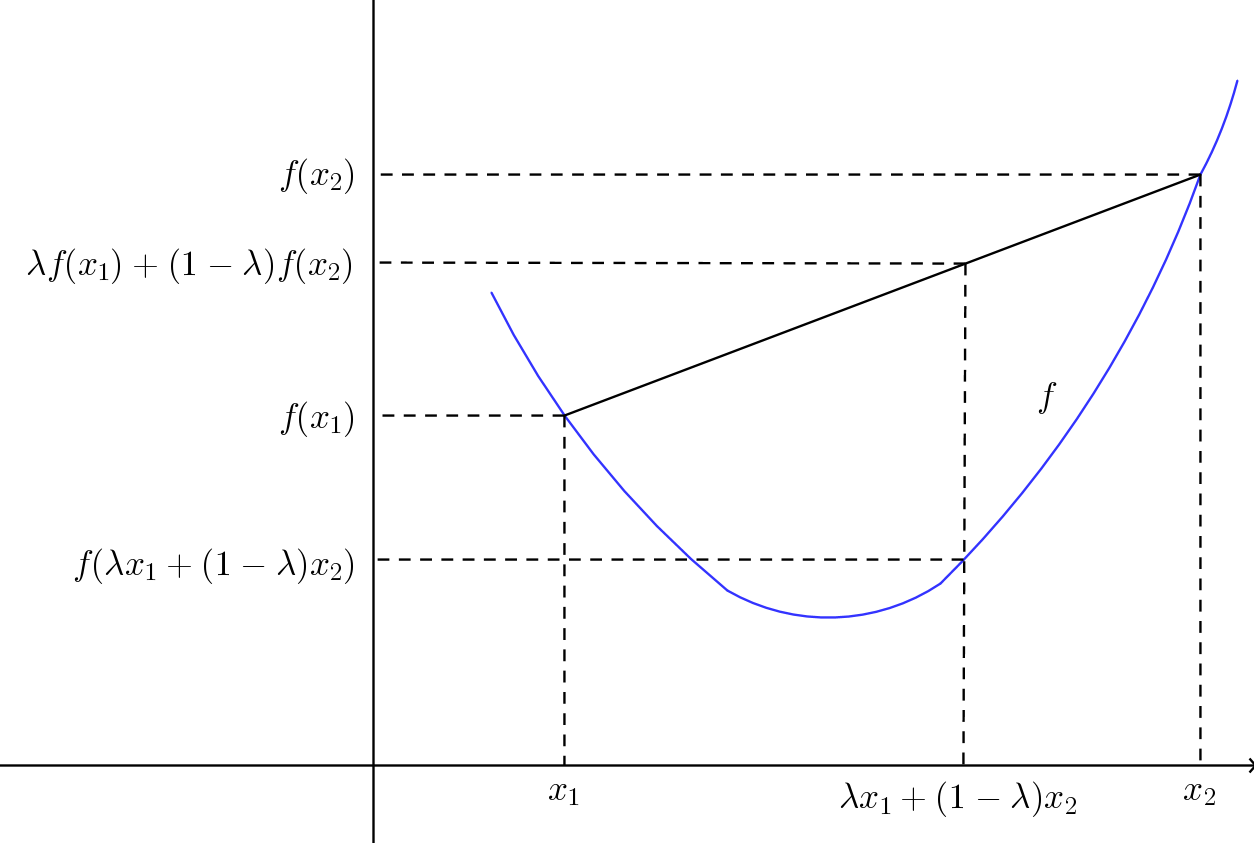
\includegraphics{./partes/sub_sec/codigo-image/f_convx.png}
   \caption{{\footnotesize Interpretaci\'on geom\'etrica de funci\'on convexa en $\mathbb{R}$ \cite{apoyo}}}
   \label{f-convx}
\end{figure}


Los siguientes son algunos ejemplos de funciones convexas.\\

\begin{enumerate}
   \item $f(x) = 3x + 4$
   \item $f(x) = |x|$
   \item $f(x) = x^2 - 2x$
   \item $f(x) =  \displaystyle \left( -x \right)^\frac{1}{2}$
   \item $f(x_1, x_2) = 2x_{1}^2 + 2x_{2}^2 - 2 x_1 x_2$
   \item $f(x_1, x_2, x_3) = x_{1}^{4} + x_{2}^{2} + 3x_{3}^{2} - 4x_1 - 4x_{2} x_{3}$
\end{enumerate}


Note que en cada uno de los ejemplos las funciones son convexas sobre $\mathbb{R}^n$. Excepto para el ejemplo 4, la funci\'on no est\'a
definida para $x < 0.$ Se pueden construir ejemplos de funciones que son convexas en una regi\'on pero no sobre $\mathbb{R}^n$. Por
ejemplo $f(x) = x^3$  no es convexa sobre $\mathbb{R}$, pero es convexa sobre $S= \{x:\, x \geqslant 0\}.$ Un ejemplo de ello es $f(x) = x^3$
no es convexa sobre $\mathbb{R}$ pero lo es sobre $S = \{x: x \geqslant 0\}.$\\ \\

De ahora en adelante nos concentraremos en funciones convexas, pues el resultado para funciones c\'oncavas puede ser obtenido f\'acilmente
notando que $f$ es c\'oncava si y s\'olo si $-f$ es convexa.\\ \\


Un conjunto asociado a una funci\'on convexa $f$ es $S_{\alpha} = \{x \in S: f(x) \leqslant \alpha \}, \,\, \alpha \in \mathbb{R}$, 
usualmente referido como {\it conjunto de nivel}. A veces este conjunto es llamado un {\it conjunto subnivel}, para
diferenciarlo del {\it conjunto supernivel} $\{ x \in S:\,  f(x) \geqslant \alpha \}$ note que \'estos tienen propiedades a 
las de una funci\'on c\'oncava. \\ \medskip

{\teorema Sea $S$ un conjunto convexo no vac\'io en $\mathbb{R}^n$ y sea $f: S \longmapsto \mathbb{R}$ una funci\'on convexa. Entonces el 
conjunto de nivel $S_{\alpha} = \{ x \in S:\, f(x) \leqslant\alpha \}; \,\, \alpha \in \mathbb{R}$ donde es un n\'umero real, es un 
conjunto convexo. \label{nivel-convx} }\\ 

\textbf{\itshape Demostraci\'on:}\\
Sean $x_1, x_2\, \in S_{\alpha}.$ Entonces $x_1, x_2\, \in S$  y  $f(x) \leqslant \alpha$  y  $f(x) = \alpha$. Ahora, sea $\lambda \in (0, 1)$
y $x = \lambda x_1 + (1 - \lambda)x_2$. Por la convexidad de $S$ se tiene que $x \in S$, por otro lado, dada la convexidad de $f$ se tiene:

$$f(x) = \lambda f(x_1) + (1 - \lambda) f(x_2) \leqslant \lambda \alpha (1 - \lambda)\alpha = \alpha$$

Por lo tanto, $x \in S_{\alpha},$ y por consiguiente, $S_{\alpha}$ es convexo.
\begin{flushright}
   $\square$
\end{flushright}

\medskip

\textbf{Continuidad de funciones convexas}\\\\

Una propiedad importante de funciones convexas y c\'oncavas es que son continuas en el interior de su dominio.\\ \\

{\teorema Sea $S$ un conjunto convexo no vac\'io en $\mathbb{R}^n$ y sea $f: S \longmapsto \mathbb{R}^n$ una funci\'on convexa. Entonces $f$
es continua en el interior de $S.$ \label{fconvex-continuos} }\\

%hacer demostracion? esta bastnte larga
% \textbf{\itshape Demostraci\'on:}\\
% Sea $\overline{x} \in \mathring{S}$. Para probar la continuidad de $f$ en $\overline{x}$, es necesario mostrar que dado $\varepsilon > 0$
% existe un $\delta > 0$ tal que $\parallel x - \overline{x} \parallel \leqslant \delta $

Note que las funciones convexas y c\'oncavas pueden no ser continuas en todo lugar. Sin embargo, por el Teorema (\ref{fconvex-continuos}), 
los puntos de discontuindad solo son permitidos en la frontera de $S$, como se ilustra en la siguiente funci\'on convexa definida en 
$S = \{ x:\, -1 \leqslant x \leqslant 1 \}$:

\[f(x) = \displaystyle{\left \{ \begin{array}{lcl}
                                  x^2 &\mbox{para}& |x| < 1\\
                                  2 &\mbox{para}& |x| = 1
                               \end{array}
\right.}\]










 %						funciones convexas
%\newpage
\subsection{Subgradiente}

Las funciones convexas poseen algunas propiedades usuales de diferenciabilidad, y una de ellas es la existencia de la derivada direccional 
lateral (derecha e izquierda) en toda direcci\'on en un punto interior de su dominio, as\'i como en el caso usual de la derivada direccional 
de una funci\'on diferenciable puede ser escrita en t\'erminos del vector gradiente, que est\'a asociado con un hiperplano tangente al
gr\'afico de la funci\'on, la derivada lateral derecha de una funci\'on convexa, no necesariamente diferenciable puede ser escrita en
t\'erminos de vectores subgradientes que est\'an asociados con hiperplanos soportes al epigrafo de la funci\'on. En lo sucesivo nos 
referiremos a la derivada direccional derecha como derivada direccional \cite{navarro}.
\medskip

{\definicion Sean $f: \mathbb{R}^n \longmapsto \mathbb{R},\, x\in \mathbb{R}^n;$ la derivada direccional de $f$ en $x$ con respecto a
$y$ es definida como el siguiente lı\'imite:


\[f'(x) = \displaystyle{\lim_{t \rightarrow 0^{+} }\dfrac{f(x + ty)- f(x)}{t}}\]

si este l\'imite existe. \label{derivada-dir}}\\

%------------------------------------epigrafo e hipografo----------------------------------------------------------

\textbf{\large Hipografo y epigrafo de una funci\'on}
\medskip

Una funci\'on $f$ en $S$ puede ser completamente descrita por el conjunto $\{[x, f(x)]:\, x \in S\} \subset \mathbb{R}^n,$ cada cual se 
refiere \textbf{\itshape grafo} de la funci\'on. Se puede construir uno de dos conjuntos que est\'an relacionados al grafo de la funci\'on 
$f:$ el {\it epigrafo} y el {\it hipografo} de $f.$
\medskip

{\definicion Sea $S$ un conjunto no vac\'io en $\mathbb{R}^n,$ y sea $f: S \longmapsto \mathbb{R}.$ El epigrafo de $f$ denotado por 
{\it epi(f),} es un subconjunto de $\mathbb{R}^{n+1}$ definido por:
$$\{(x, y):\, x \in S,\,  y \in \mathbb{R},\, y \geqslant f(x)\}$$

El {\it hipografo} de $f$ denotado por {\it hyp(f)} es un subconjunto de $\mathbb{R}^{n+1}$ definido por:
$$\{(x, y):\, x \in S,\, y \in \mathbb{R},\, y \leqslant f(x)\}$$  \label{epi-hipo}}

\begin{figure}
   \centering
   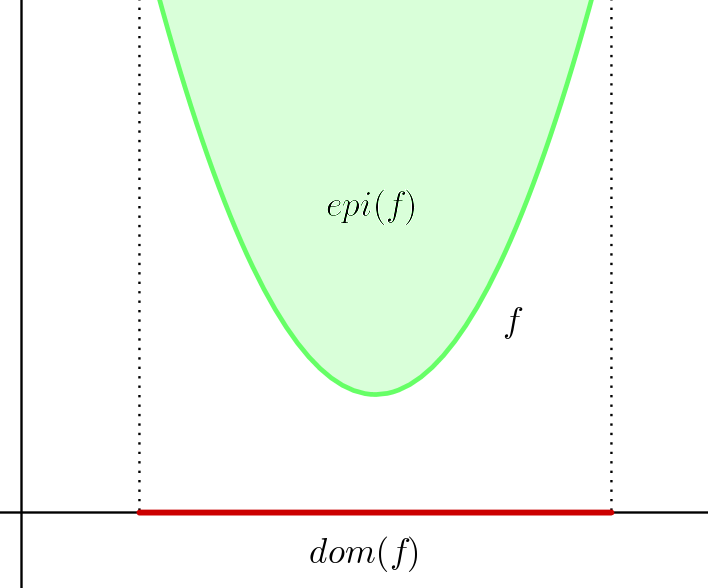
\includegraphics{./partes/sub_sec/codigo-image/epi.png}
   \caption{Epigrafo de una funci\'on $f$ en $\mathbb{R}$ \cite{lara}}
\end{figure}

{\teorema Sea $S$ un conjunto convexo no vac\'io en $\mathbb{R}^n,$ y sea $f: S \longmapsto \mathbb{R}.$ Entonces $f$ es convexa si y solo si
el $epi(f)$ es un conjunto convexo.\label{epi-convx}} \medskip


%-------------------------------------fin de epi e hipo------------------------------------------------------------

{\definicion Sean $f: \mathbb{R}^n \longmapsto \mathbb{R},\,\, x_0 \in \mathbb{R}^n$ Un vector $\vec{s} \in \mathbb{R}^n$ tal que:
$$f(x) \geqslant f(x_{0}) + \langle s, x - x_0 \rangle,\,\, \forall x\in \mathbb{R}^n$$

es llamado un subgradientede $f$ en $x_0$ \cite{navarro}  \label{subgradiente}}\\

El conjunto de subgradientes de una funci\'on $f$ en el punto $x_0$ es llamado subdiferencial de $f$ en $x_0$ y se denota por 
$\partial f(x_0).$
\medskip

{\definicion Si $\partial f(x_0) \neq \emptyset$ diremos que $f$ es diferenciable en $x_0.$ \label{sub-dif}}\\


Geom\'etricamente, $s \in \mathbb{R}^n$ es un subgradiente de la funci\'on convexa $f$ en $x_0$ si el gr\'afico de $f$ en $\mathbb{R}^{n+1}$
est\'a por encima del gr\'afico del hiperplano $y = f(x) + \langle s, x - x_0 \rangle .$ Como $(x_0, f(x_0))$ est\'a en el hiperplano, este 
hiperplano constituye un hiperplano soporte a $epi(f)$ en $(x_0, f(x_0)).$ Esto es, la existencia de un vector subgradiente establece la
existencia de un hiperplano soporte no vertical a $epi(f)$ en $(x_0, f(x_0)).$

\begin{figure}
   \centering
   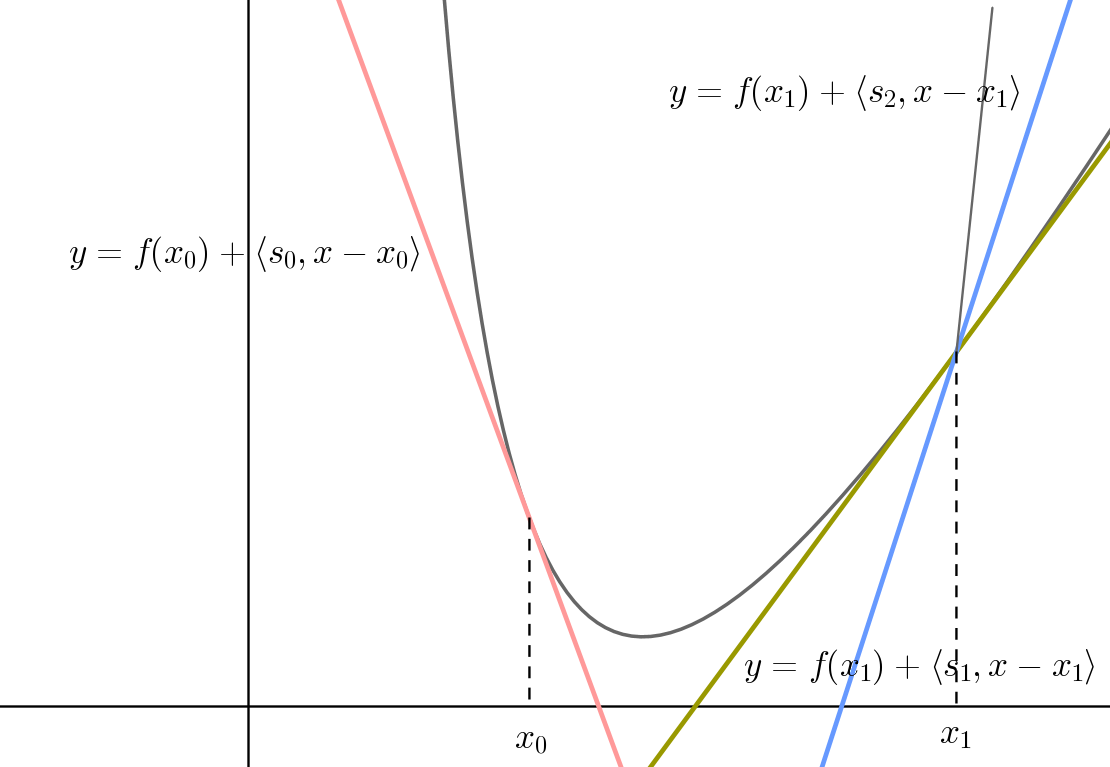
\includegraphics{./partes/sub_sec/codigo-image/subgradiente.png}
   \caption{Interpretaci\'on geom\'etrica del subgradiente en $\mathbb{R}$ \cite{navarro}}
\end{figure}

El siguiente teorema establece que toda funci\'on convexa es subdiferenciable en el interior de su dominio \cite{navarro}.

{\teorema Sea $f$ una funci\'on convexa definida en un convexo $S,$ entonces en cada punto $x_0 \in \mathring{S}$ se tiene que
$\partial f(x_0) \neq \emptyset$ \label{convx-int}}
\medskip

El rec\'iproco del teorema anterior es falso, pues la condici\'on de ser punto interior es indispensable, por ejemplo, si se considera la
funci\'on convexa $f:[0, \infty ) \longmapsto \mathbb{R}$ dada por $f(x) = - \sqrt{x}$ entonces se tiene que $\partial f(0) = \emptyset$
\newpage







 %						subgradiente
%\newpage
\subsection{Funciones convexas diferenciables}

{\definicion \cite{no-lineal} Sea $S$ un conjunto no vac\'io en $\mathbb{R}^n,$ y sea $f: S \longmapsto \mathbb{R}.$ Entonces $f$ se dice que es diferenciable
en $\overline{x} \in \mathring{S}$ si existe un vector $\nabla f(\overline{x}),$ llamado vector gradiente; y una funci\'on
$\alpha: \mathbb{R}^n \longmapsto \mathbb{R}$ tal que:

$$f(x) = f(\overline{x}) + \nabla f(\overline{x})^t (x - \overline{x}) + \parallel x - \overline{x} \parallel
\alpha \langle \overline{x}; x - \overline{x}\rangle \,\,\, \forall \, x \in S$$

d\'onde $\displaystyle{\lim_{x \rightarrow \overline{x}} \alpha \langle \overline{x}, x - \overline{x} \rangle = 0.}$ \label{def-dif}}
\medskip

La funci\'on $f$ se dice que es diferenciable en $S' \subseteq S$ si \'esta es diferenciable en cada punto de $S'.$ Esta representaci\'on de 
$f$ es llamada {\it expansi\'on (serie de Taylor) de primer orden} de $f$ en el punto $\overline{x}.$
\\
Note que si $f$ es diferenciable en $\overline{x},$ solo podr\'ia haber un vector gradiente el cual est\'a dado por:

$$\nabla f(\overline{x}) = \left( \dfrac{\partial f(\overline{x})}{\partial x_1}, \dots , 
\dfrac{\partial f(\overline{x})}{\partial x_n}\right)^t \equiv (f_1(\overline{x}), \ldots , f_n(\overline{x}))^t$$

d\'onde $f_i(\overline{x}) = \dfrac{\partial f(\overline{x})}{\partial x_i}$ es la derivada parcial de $f$ respecto a $x_i$ en $\overline{x}$.
\medskip

{\teorema Sea $f$ una funci\'on convexa definida en un conjunto convexo $S$ de $\mathbb{R}^n$ y sea $x$ un punto interior de $S.$ $f$ es 
diferenciable en $x$ si y s\'olo si posee un \'unico subgradiente en $x.$ En tal caso $\partial f(x) = \{\nabla f(x)\}.$ 
\label{one-subgradiente} }

%revisar la importacia de los teoremas anteriores para llegara este resultado. Non linear programacion
\medskip

{\teorema Sea $S$ un conjunto abierto no vac\'io en $\mathbb{R}^n$ y sea $f: S \longmapsto \mathbb{R}$ diferenciable en $\mathbb{R}$. Entonces
$f$ es convexa si y s\'olo si para cualquier $\overline{x} \in S$ se tiene:
$$f(x) \geqslant f(\overline{x}) + \nabla f(\overline{x})^t(x - \overline{x})\,\,\,\, \forall x \in S$$

De igual forma, $f$ es estrictamente convexa si y s\'olo si para cada $x \in S$ se tiene:
$$f(x) > f(\overline{x}) + \nabla f(\overline{x})^t(x - \overline{x})\,\,\,\, \forall x \neq \overline{x} \in S$$ \label{carac1}}
\medskip

El siguiente teorema da una carcterizaci\'on suficiente y necesaria para funciones convexas. Para una funci\'on $f$ de una variable, la 
caracterizaci\'on se reduce a una pendiente creciente.\\ 

{\teorema Sea $S$ un conjunto abierto no vac\'io en $\mathbb{R}^n$ y sea $f: S \longmapsto \mathbb{R}$ diferenciable en $S.$ Entonces $f$ es
convexa si y s\'olo si para cada $x_1, x_2 \in S$ se tiene:
$$[\nabla f(x_2) - \nabla f(x_1)]^t (x_2 - x_1) \geqslant 0.$$

Similarmete, $f$ es esrictamente convexa para cualquier $x_1, x_2 \in S$ distintos, entonces se tiene:
$$[\nabla f(x_2) - \nabla f(x_1)]^t (x_2 - x_1) \geqslant 0.$$ \label{carac2}}
\medskip

Aunque los teoremas (\ref{carac1}) y (\ref{carac2}) dan una caracterizaci\'on suficiente y necesaria para funciones convexas, comprobar
estas condiciones desde el punto de vista computacional es muy dif\'icil. Una caracterizaci\'on m\'as simple y manejable, al menos para 
funciones cuadr\'aticas puede obtenerse siempre que la funci\'on sea dos veces diferenciable. \\ \

\textbf{Funciones dos veces diferenciables} \cite{no-lineal}\\
\medskip

Una funci\'on $f$ que es diferenciable en $\overline{x}$ se dice que es dos veces diferenciable en $\overline{x}$ si la representaci\'on de la
{\it expansi\'on de segundo orden (serie de Taylor)} de la siguiente definici\'on existe.\\ 
\medskip

{\definicion Sea $S$ un conjunto no vac\'io en $\mathbb{R}^n$ y sea $f: S \longmapsto \mathbb{R}.$ Entonces $f$ se dice que es {\itshape dos
veces diferenciable} en $\overline{x} \in \mathring{S}$ si existe un vector $\nabla f(\overline{x}),$ y una matriz sim\'etrica 
$H( \overline{x} )$ de $n \times n,$ llamada {\bf{\itshape matriz hessiana}} y una funci\'on $\alpha:\mathbb{R}^n \longmapsto \mathbb{R}$ tal que:

$$f(x) = f(\overline{x}) + \nabla f(x)^t (x-\overline{x}) + \dfrac{1}{2} (x-\overline{x}) H(\overline{x}) (x-\overline{x}) + 
\parallel x-\overline{x} \parallel ^2 \alpha \langle \overline{x}, x-\overline{x} \rangle$$

para cada $x \in S,$ donde $\displaystyle{\lim_{x\longmapsto \overline{x}} \alpha \langle \overline{x}, x-\overline{x} \rangle = 0}.$ \\
La funci\'on $f$ se dice dos veces diferenciable en el conjunto abierto $S' \subseteq S$ si es dos veces diferenciable en cada punto de $S'.$
\label{dos-dif}} \\

Cabe se\~nalar que para funciones dos veces diferenciables, la matriz hessiana $H(\overline{x})$ est\'a compuesta por las derivadas parciales
de orden dos $f_{ij}(\overline{x}) \equiv \dfrac{\partial^2 f(\overline{x})}{\partial x_i \partial x_j};\,\, i = 1, \ldots , n.
\,\, j=1,\ldots , n$ y est\'a dada de la siguiente forma:

\[H(\overline{x}) = \begin{bmatrix}
                       f_{11}(\overline{x}) & f_{12}(\overline{x}) & \ldots & f_{1n}(\overline{x})\\
                       f_{21}(\overline{x}) & f_{22}(\overline{x}) & \ldots & f_{2n}(\overline{x})\\
                       \vdots               &  \vdots 		   & \ddots &  \vdots \\
                       f_{n1}(\overline{x}) & f_{n2}(\overline{x}) & \ldots & f_{nn}(\overline{x})
                    \end{bmatrix}
\]


~ \medskip


 %						funciones convexas diferenciables
%\newpage
\subsection{Mínimo y máximo de funciones convexas}
~\medskip

En esta parte se considerarán problemas de minimizar y maximizar una función convexa sobre un conjunto convexo y se desarrollaran las 
condiciones necesarias y suficientes para optimalidad \cite{no-lineal}.\\ 
\medskip
\

{\definicion Sea $f: \mathbb{R}^n \longmapsto \mathbb{R}$ y consideremos el problema a minimizar $f(x)$ sujeto a $x \in S.$ Un punto $x \in S$ 
es llamado \textbf{\itshape solución factible} para el problema. Si $\overline{x} \in S $ y $ f(x) \geqslant f(\overline{x})$ para cada $x \in 
S,\,\, \overline{x} $ es llamado una \textbf{\itshape solución optima, solución optima global} o simplemente una \textbf{\itshape solución}
para el problema. \label{sol-problem}  }\\

La colección de soluciones óptimas es llamada \textbf{\itshape solución óptima alternativa.} 
\begin{itemize}
   \item Si $\overline{x} \in S$ y si existe un $\varepsilon-$vecindario $N_{\varepsilon}(\overline{x})$ alrededor de $\overline{x}$ tal que $ f(x) \geqslant f(\overline{x})$ para
	 cada $x \in S \cap N_{\varepsilon}(\overline{x}), \,\, \overline{x} $ es llamado \textbf{\itshape solución óptima local.}
   \item Si $\overline{x} \in S$ si $ f(x) > f(\overline{x})$ para todo $ x \in S \cap N_{\varepsilon}(\overline{x}), \,\,
	 x \neq \overline{x}$ para algún $\varepsilon > 0,\,\, \overline{x} $ es llamada \textbf{\itshape solución óptima local estricta}.
   \item Si $\overline{x} \in S$ es el único mínimo local en $ S \cap N_{\varepsilon}(\overline{x}), $ para algún vecindario
	 $N_{\varepsilon}(\overline{x})$ alrededor de $\overline{x}, \,\, x\,$ es llamada \textbf{\itshape solución óptima local fuerte o 
	 aislada}
\end{itemize}
~\medskip

Todos estos tipos de \'optimo local o m\'inimo local a veces tambi\'en se denominan como \textbf{\itshape m\'inimo relativo.} La 
Figura(\ref{mins}) ilustra ejemplos de m\'inimos locales y globales para el problema de minimizar $f(x)$ sujeto a $x \in S$

\begin{figure}
   \centering
   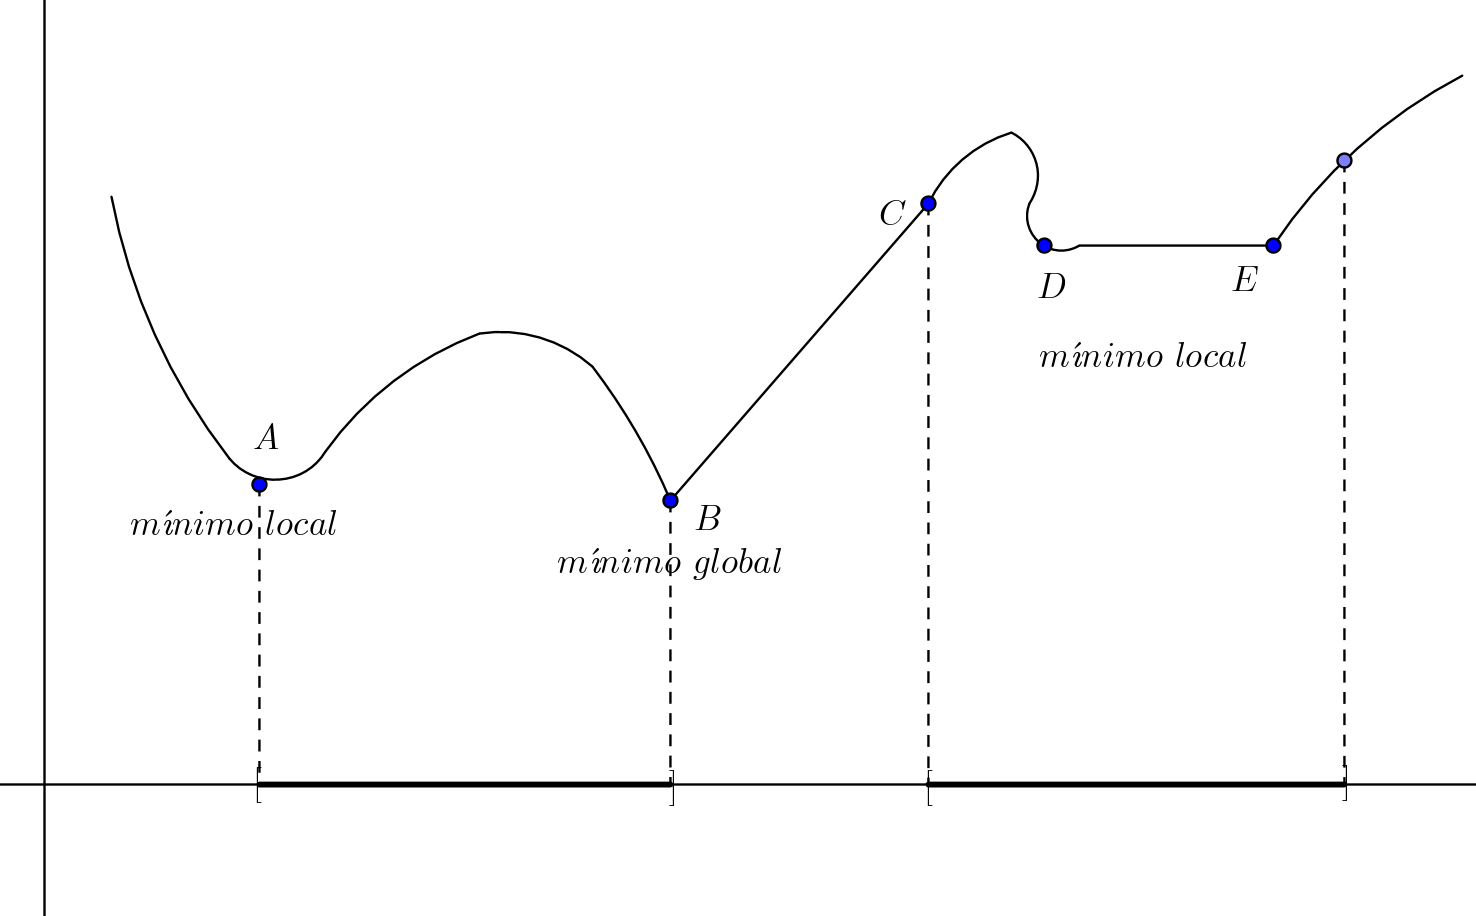
\includegraphics{./partes/sub_sec/codigo-image/minimos.png}
   \caption{M\'inimo local y global \cite{no-lineal}}
   \label{mins}
\end{figure}
\medskip

{\teorema Sea $S$ un conjunto convexo no vac\'io en $\mathbb{R}^n$ y sea $f: S \longmapsto \mathbb{R}$ convexa en $S.$ Considere minimizar el
problema $f(x)$ sujeto a $x \in S.$ Suponga que $\overline{x} \in S$ es una soluci\'on \'optima local para el problema, entonces:
\begin{enumerate}
   \item $\overline{x}$ es una soluci\'on \'optima global.
   \item Si $\overline{x}$ es una soluci\'on m\'inima estricta o $f$ es estrictamente convexa, $\overline{x}$ es la \'unica soluci\'on 
	 \'optima global y tambi\'en es un m\'inimo local.
\end{enumerate} \label{teo1-sol}}
~ \medskip

Acontinuaci\'on, se presenta una condici\'on necesaria y suficiente para la existencia de una soluci\'on global. Si tal soluci\'on \'optima no
existe, entonces $\inf \{f(x): x \in S \}$ es finito, pero no se alcanza en ning\'un punto de $S$ \'o es igual a $- \infty.$

{\teorema Sea $f$ una funci\'on convexa en $\mathbb{R}^n$ y $S$ un conjunto convexo en $\mathbb{R}^n$ Consideremos el problema de 
optimizaci\'on
\[\displaystyle{\min_{_{x \in S}} f(x)}\]

Entonces $\overline{x}$ es un m\'inimo local de $f$ sobre $S$ si y s\'olo si existe $s \in \partial f(\overline{x})$ tal que
\[\langle s, x - \overline{x} \rangle \geqslant 0 \,\, \mbox{ para toda } \, x \in S\]  \label{teo-important}}
\medskip

\textbf{Maximizar una funci\'on convexa}\\
\

Se desarrollar\'a una condici\'on necesaria para un m\'aximo de una funci\'on convexa sobre un conjunto convexo. Desafortunadamene, esta
condici\'on no es suficiente. Por lo tanto, es improbable, que varios m\'aximos que satisfagan la condici\'on del Teorema \ref{teo-max} 
existan. En el caso de mimizar, no existe informaci\'on local de tales soluciones que podr\'ian llevar a mejores puntos. Por lo tanto, 
maximizar una funci\'on convexa es una tarea mucho m\'as dura que minimizar una funci\'on convexa.\\ \\

{\teorema Sea $f: \mathbb{R}^n \longmapsto \mathbb{R}$ una funci\'on convexa y sea $S$ un conjunto convexo no vac\'io en $\mathbb{R}^n.$
Considere el problema:
\[\max_{{x \in S}} f(x)\]
Si $\overline{x} \in S$ es una soluci\'on \'optima local 
\[\langle s, x - \overline{x} \rangle \leqslant 0\]

para cada $x \in S$, donde $s \in \partial f(\overline{x})$ \label{teo-max}}




 %						minimo y maximo de funciones convexas

%\subsection{Propiedades topol\'ogicas de los conjuntos convexos}














